An \textbf{RTOS} (Real-time Operating System) must meet the same requirements as a standard general purpose operating system (GPOS) and offers services for

\os{\begin{itemize}
\item Task Management
\item Resource Management
\item Communication
\item Synchronization
\item Protection
\end{itemize}
\newpage
}

\nsl{\begin{itemize}
\item  \textbf{Task Management: }This is the management and organization of the implemented programs to be processed, also called tasks. The mission of the task management is thus essentially in the allocation of the processor (or the processors in a multiprocessor system) to the task.
\item  \textbf{Resource Management: }Tasks need resources for their execution, their allocation is the task of resource management. This mainly includes:- Memory management, responsible for allocating memory- Input/Output (I/O) management responsible for the allocation of I/O devices to  the tasks.
\item  \textbf{Communication: }The communication between tasks, called inter-process communication.
\item  \textbf{Synchronization: }A special form of communication is the synchronization, which refers to the timing of the tasks.
\item  \textbf{Protection: }The protection of resources against unauthorized access by tasks.
\end{itemize}}

These traditional requirements are exactly the same RTOSes as with GPOSes. Depending on the application, some of the services might be implemented only  rudimentary or completely absent. This is in particular with \textbf{embedded} \textbf{systems}, where the \textbf{RTOS} is kept as \textbf{lean as possible}, due to the limited resources.\\

In addition to the traditional OS requirements, real-time operating systems are required to 

\begin{itemize}
	\item  Respect for \textbf{timeliness} and \textbf{concurrency}
	\item  Respect for \textbf{availability}
\end{itemize}

These requirements of RTOS dominate the other requirements, even if compromises are necessary.

\section{Structure of an RTOS}

A real-time operating system (RTOS) is a program that schedules execution in a timely manner, manages system resources, and provides a consistent foundation for developing application code.\\

Early operating systems had a monolithic structure, i.e. all functionality was implemented in a uniform, not further subdivided software block. This led to a number of disadvantages such as poor maintainability, poor adaptability and high error rate. Today's operating systems therefore follow a hierarchical layers model. 

	\begin{figure}[h]
    \centering
    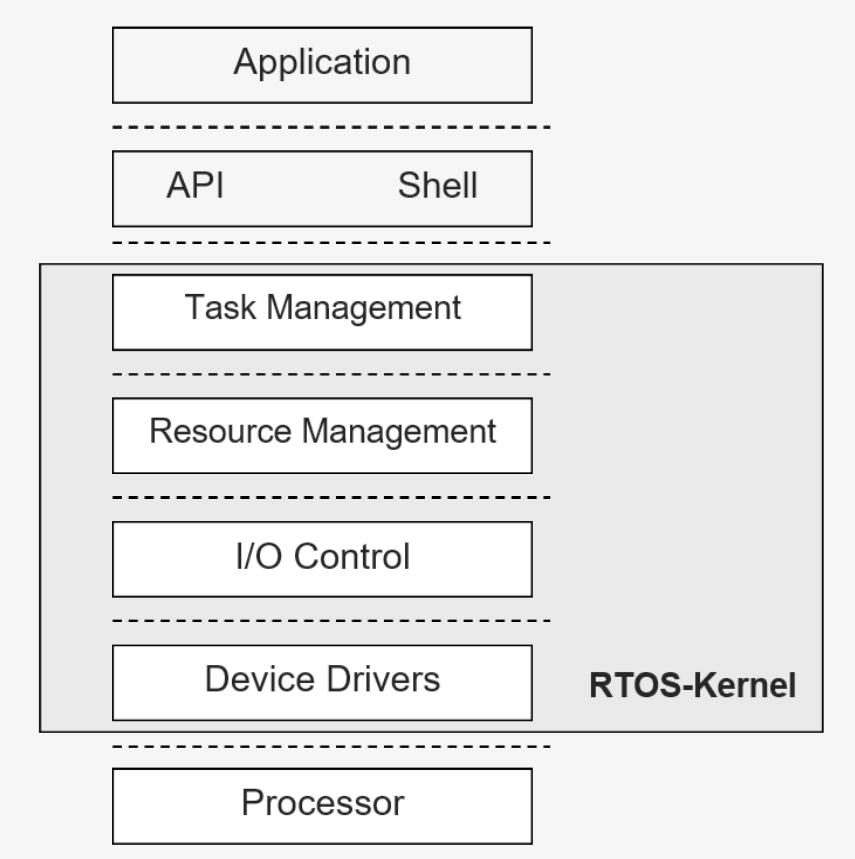
\includegraphics[width=9cm, height=7cm]{Images/image79.png}
    %\caption{}
    \label{fig:Fig 25}
    \end{figure}

\begin{itemize}
	\item  \textbf{Device Driver: } This layer abstracts from the hardware, and
	\begin{itemize}
		\item realizes the \textbf{hardware-dependent} \textbf{control} of each device
		\item realizes the \textbf{hardware-independent} interface for the above layer. 
	\end{itemize}

		Ideally, the device drivers are the only hardware dependent layer in the OS. When adapting to other devices, only the device driver layer must be changed.
	\item  \textbf{I/O (Input-/Output) Control}, realizes the logical, hardware-independent device control. 
	\item  \textbf{Resource Management: } responsible for (allocation) and de-allocation (release) of memory and I/O resources.
	\item  \textbf{Task Management: } Responsible for the allocation of the processor to each task. 
	\item  \textbf{API (Application Program Interface): } Realizes the interface to the application.
\end{itemize}

The OS kernel is critical for the stability and security, it is executed in the so-called \textbf{kernel mode} of the processor, which allows full access to all resources.

\begin{itemize}
\item The \textbf{kernel mode} is a special operating mode of (advanced) microprocessors, enabling privileged instructions, direct access to memory and I/O, change configuration registers, etc.
\item In normal \textbf{user mode} this privileged commands are blocked so that an application can not interfere with important operating system parts. This is one of the protection services of the operating system.
\item In the previous layer model, the core operating system extends over the layers 1 -- 4. Since the core contains many layers, it is called a \textbf{macro core operating system}.
\item Today's RTOSes must be highly configurable, especially in the field of \textbf{embedded systems} where scarce resources are typical  $\rightarrow$ FreeRTOS.
\item It is therefore desirable to remove unwanted parts from the operating system, e.g. not needed scheduling or protection methods. This leads to the concept of the \textbf{micro-kernel operating system}.
\end{itemize}

\section{Task Management}

The task management is a core task of operating systems. The most significant differences between standard and real-time operating systems are found here.\\

The tasks in a real-time application must meet the requirements for \textbf{timeliness} and \textbf{concurrency}. This requires scheduling strategies for RTOSes different from those found in  standard operating systems.\\
\os{\newpage}

{\rot\bf Task Model}\\

A \textbf{computational process} or \textbf{process} (also called \textbf{task}) is running as a computer program together with all the variables (including register states) and resources  $\rightarrow$ each process has a \textbf{main()}\\

A task is a process controlled by the RTOS for execution of a sequential program. Several tasks are being processed by the quasi-parallel processor, necessary changes between tasks are made by the RTOS' task scheduler.\\

Changes between tasks are needed to meet all tasks requirements for timeliness.

	\begin{figure}[h]
    \centering
    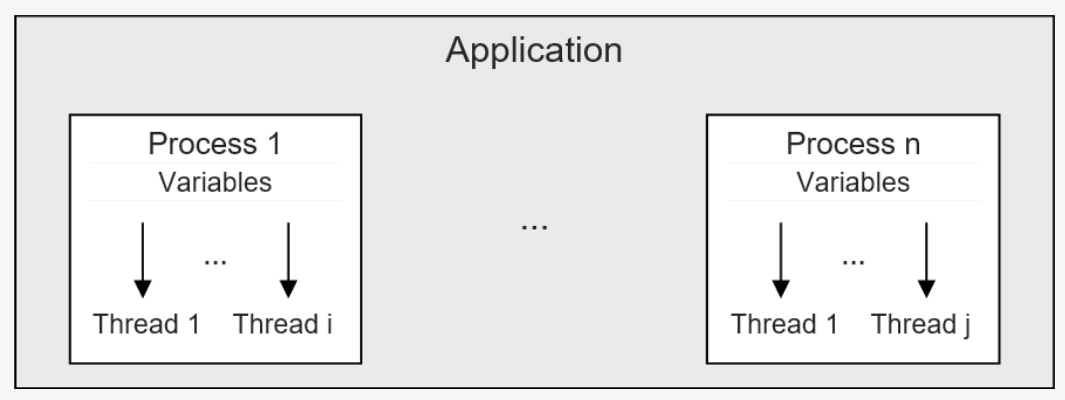
\includegraphics[width=10cm, height=4cm]{Images/image80.png}
    %\caption{}
    \label{fig:Fig 26}
    \end{figure}

Within a \textbf{\textit{process}}, there can be parallel \textbf{\textit{threads}} (running simultaneously). \\

A \textbf{\textit{thread}} must share its resources with other \textbf{\textit{threads}} of the same \textbf{\textit{process}} $\rightarrow$  just${}_{\ }$1${}_{\ }$\textbf{main()}\\

A \textbf{task} is called a \textbf{heavyweight process, }if it contains its own variables and resources separated from other tasks by the OS. It has its own address space and can communicate with other tasks via interprocess communication. \\

$\rightarrow$ A task realized as a process provides maximum protection, possible interference by other tasks is limited to predefined channels. \\

$\rightarrow$ A change of the processor to another task (\textbf{context switch}) is due to the separate resources, which is a time-consuming task.\\

A \textbf{task} realized as a \textbf{thread} is called a \textbf{lightweight process} that exists within a single process. It uses the variables and resources of the process. All threads within a process \textbf{share the same address space}. Communication can take place over any global variable within the process.

\begin{itemize}
	\item Threads can interfere with any other thread within a task.
	\item Shared memory allows great efficiency.
	\item Communication between threads is more direct and faster
	\item Context switch can take place very quickly, e.g.: FreeRTOS, VxWorks
	\item Low data protection between data of individual threads
\end{itemize}

To fulfil the \textbf{real-time requirements}, efficiency is usually more important than protection. Many real-time applications use \textbf{threads within a single task}.\\

\nsl{Often, a real-time application is realized by a \textbf{\textit{single}} \textbf{\textit{process}}, which contains threads to realize numerous tasks.\textbf{ Embedded systems} are often based on the \textbf{thread concept}, due to scarce resources.\\}

From the perspective of the real-time conditions (timeliness, concurrency, availability), \textbf{threads} aren't different from \textbf{processes}, both are usually identified by the term \textbf{task}.\\

{\rot\bf Multitasking, Context Switch }\\

Multitasking is the ability of the OS to handle multiple tasks within set deadlines. An RTOS kernel might have 2 tasks that it has to schedule to run. At certain times, execution of Task 1 has to switch to Task 2

	\begin{figure}[h]
    \centering
    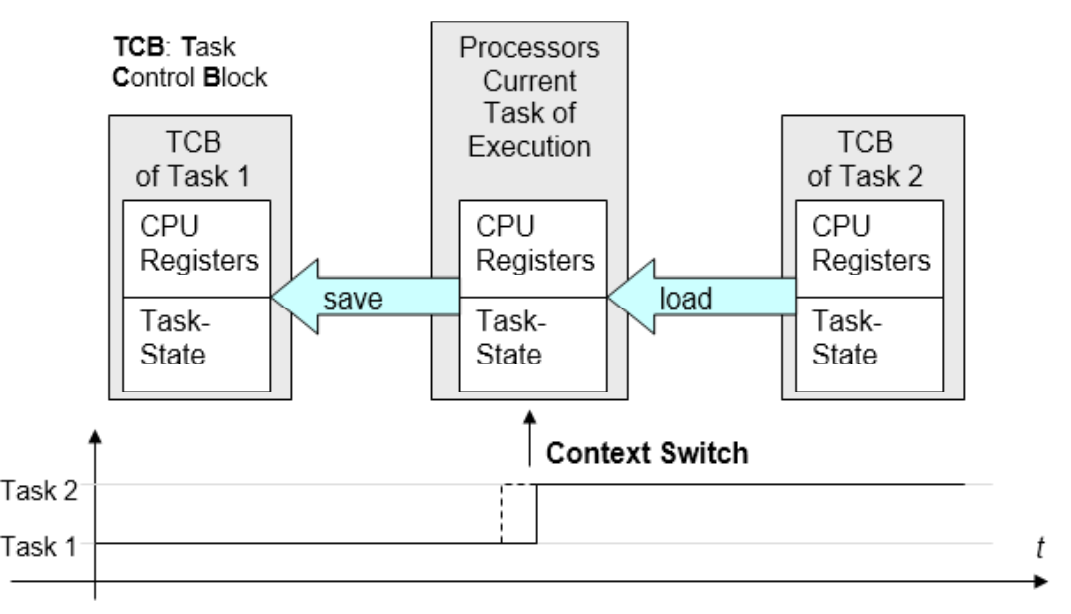
\includegraphics[width=13cm, height=6cm]{Images/image81.png}
    %\caption{}
    \label{fig:Fig 27}
    \end{figure}
\os{\newpage}

{\rot\bf Task States}\\

For each task (or threads) one can define 6 different states:

	\begin{figure}[h]
    \centering
    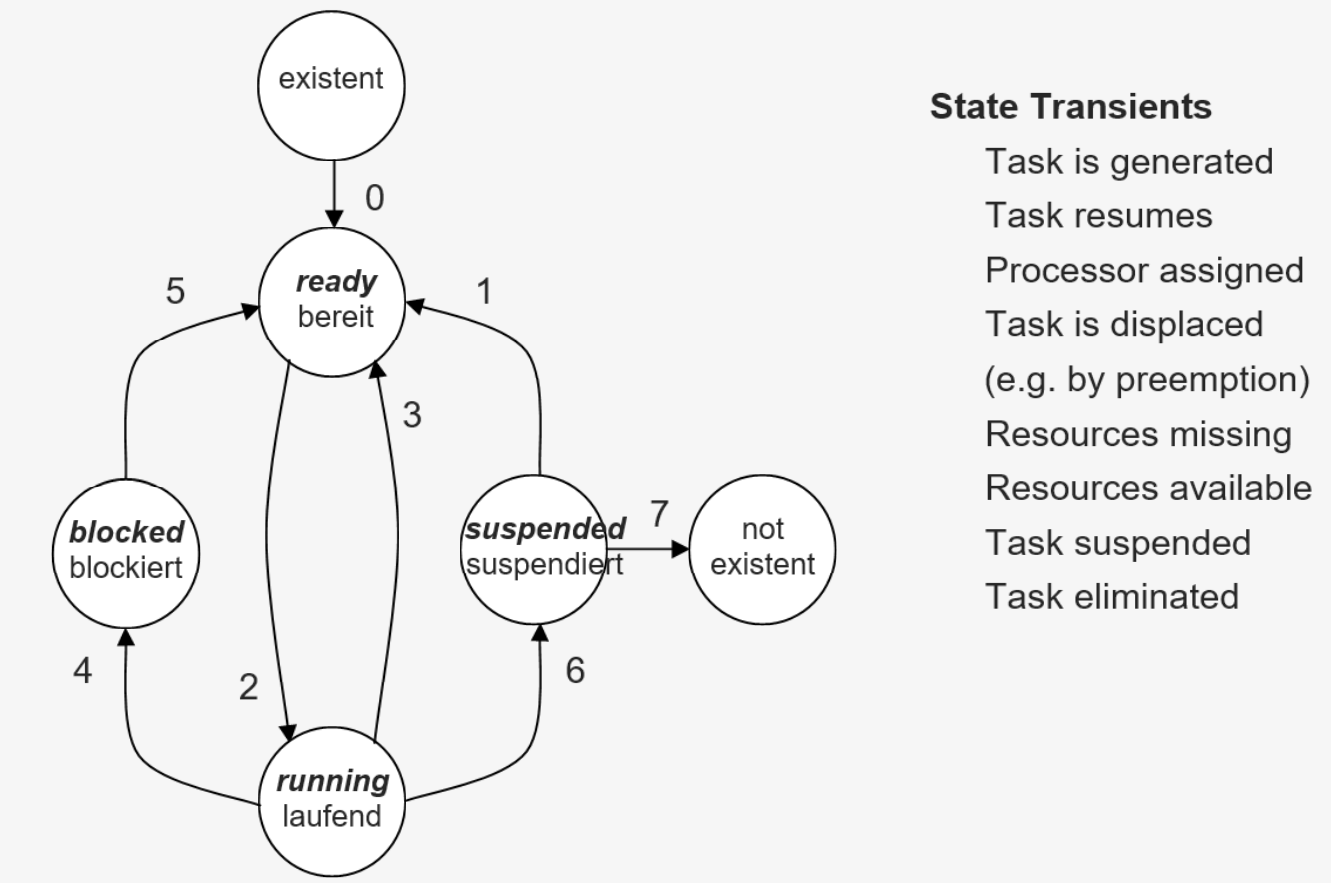
\includegraphics[width=13cm, height=8cm]{Images/image82.png}
    %\caption{}
    \label{fig:Fig 28}
    \end{figure}
\os{\newpage}
\begin{itemize}
	\item  \textbf{existent}
	\item \textbf{ ready (}waiting\textbf{)}The task is ready, all conditions are fulfilled, resources are allocated, the task is waiting for the allocation of the processor.
	\item  \textbf{running }(executing)The task is run on the processor. In a uniprocessor only one task can be in this condition, in a multi-processor system, several tasks can be in this state simultaneously. 
	\item  \textbf{blocked} (blocked)The task is waiting for an event (e.g. an input value, an inter-process communication object) or the release of a resource (task synchronization). 
	\item  \textbf{suspended }(finished)A task is suspended from its normal operations by another task. It can be resumed later
	\item  \textbf{not existent}
\end{itemize}

\section{Real-Time Scheduling}

The main job of an RTOS task management is the allocation of the processor to the ready tasks. There are different strategies, so-called scheduling strategies.\\

A \textbf{real-time scheduler} must divide all ready (runnable) tasks to the processor, so that all time conditions are met. The set of tasks managed by the real-time scheduler is called \textbf{taskset}.\\

For the evaluation of various scheduling strategies, the processor demand \textit{H} (\textbf{utilization}) is an important quantity for the load of the processor, it is defined as

\begin{equation}
	H = \frac{Demanded Processor Time}{Available Processor Time}
\label{EQ 3}
\end{equation}
\newline
Each CPU can be utilized up to 100 \% at maximum.\\

\textbf{Example}: A periodic task 1 with a period of \textit{T}${}_{P1}$ = 200 ms and an execution time of \textit{T}${}_{e1}$ = 100 ms causes a processor demand of \textit{H}${}_{1}$ = 50 \%

	\begin{figure}[h]
    \centering
    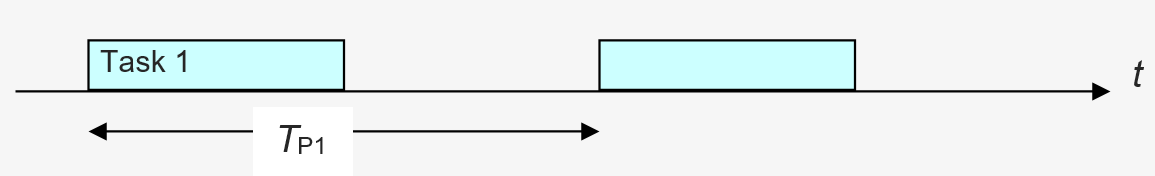
\includegraphics[width=10cm, height=2cm]{Images/image83.png}
    %\caption{}
    \label{fig:Fig 29}
    \end{figure}
\nsl{\newpage}
A second periodic task with a period of \textit{T}${}_{P2}$ = 100 ms and an execution time of \textit{T}${}_{e2}$ = 50 ms also causes a processor demand of \textit{H}${}_{2}$ = 50 \%.

	\begin{figure}[h]
    \centering
    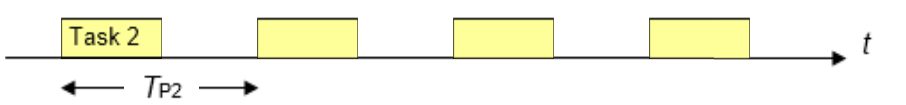
\includegraphics[width=10cm, height=2cm]{Images/image84.png}
    %\caption{}
    \label{fig:Fig 30}
    \end{figure} 

An implicit timing condition for each periodic task is: task execution must be finished before the next period starts (deadline) !\\

Both tasks cause a total processor demand \textit{H} = \textit{H}${}_{1}$ + \textit{H}${}_{2}$ = 100~\%.
\os{\newpage}
	\begin{figure}[h]
    \centering
    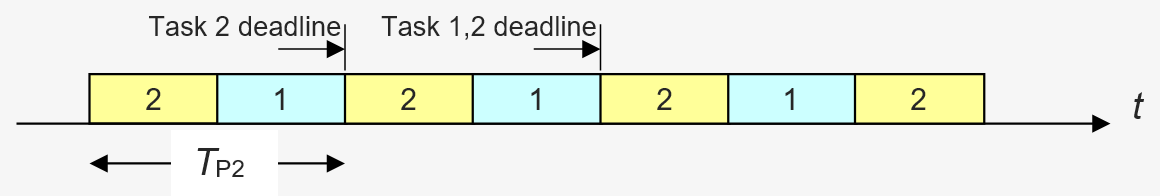
\includegraphics[width=10cm, height=3cm]{Images/image85.png}
    %\caption{}
    \label{fig:Fig 31}
    \end{figure} 
    
One possible schedule for executing both tasks is to displace task 1 after exactly half of its execution time by task 2, which is never displaced. Thus, task 1 must be displaceable:

	\begin{figure}[h]
    \centering
    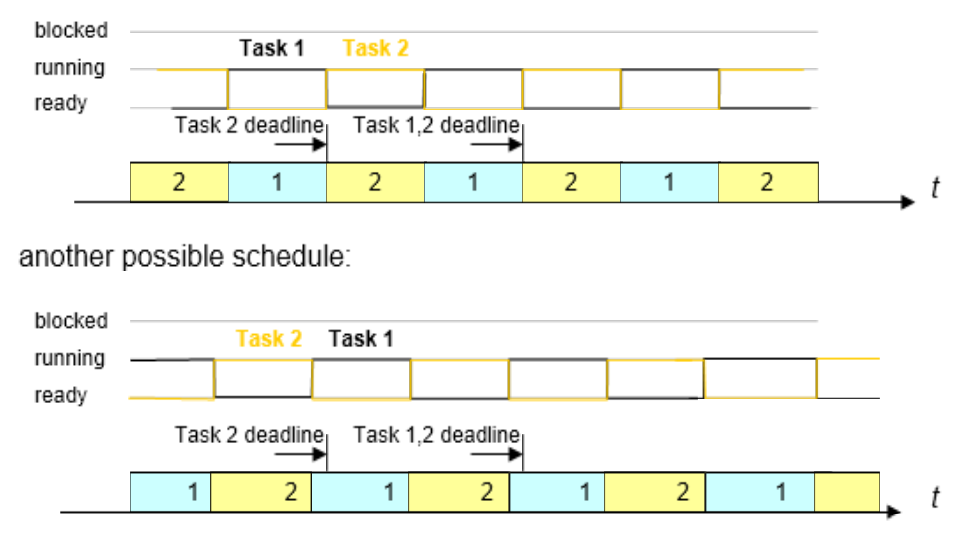
\includegraphics[width=12cm, height=6cm]{Images/image86.png}
    %\caption{}
    \label{fig:Fig 32}
    \end{figure} 
\os{\newpage}
In general, for a tasklet of \textit{n} periodic tasks, the total processor demand

\begin{equation}
	H=\sum _{i=1}^{n}\frac{T_{ei} }{T_{pi}}
\label{EQ 3}
\end{equation}

$T_{ei}$ execution time of task i, $T_{pi}$ periodic time of task i\\
\newpage

{\rot\bf Classification of Scheduling Algorithms}

	\begin{figure}[h]
    \centering
    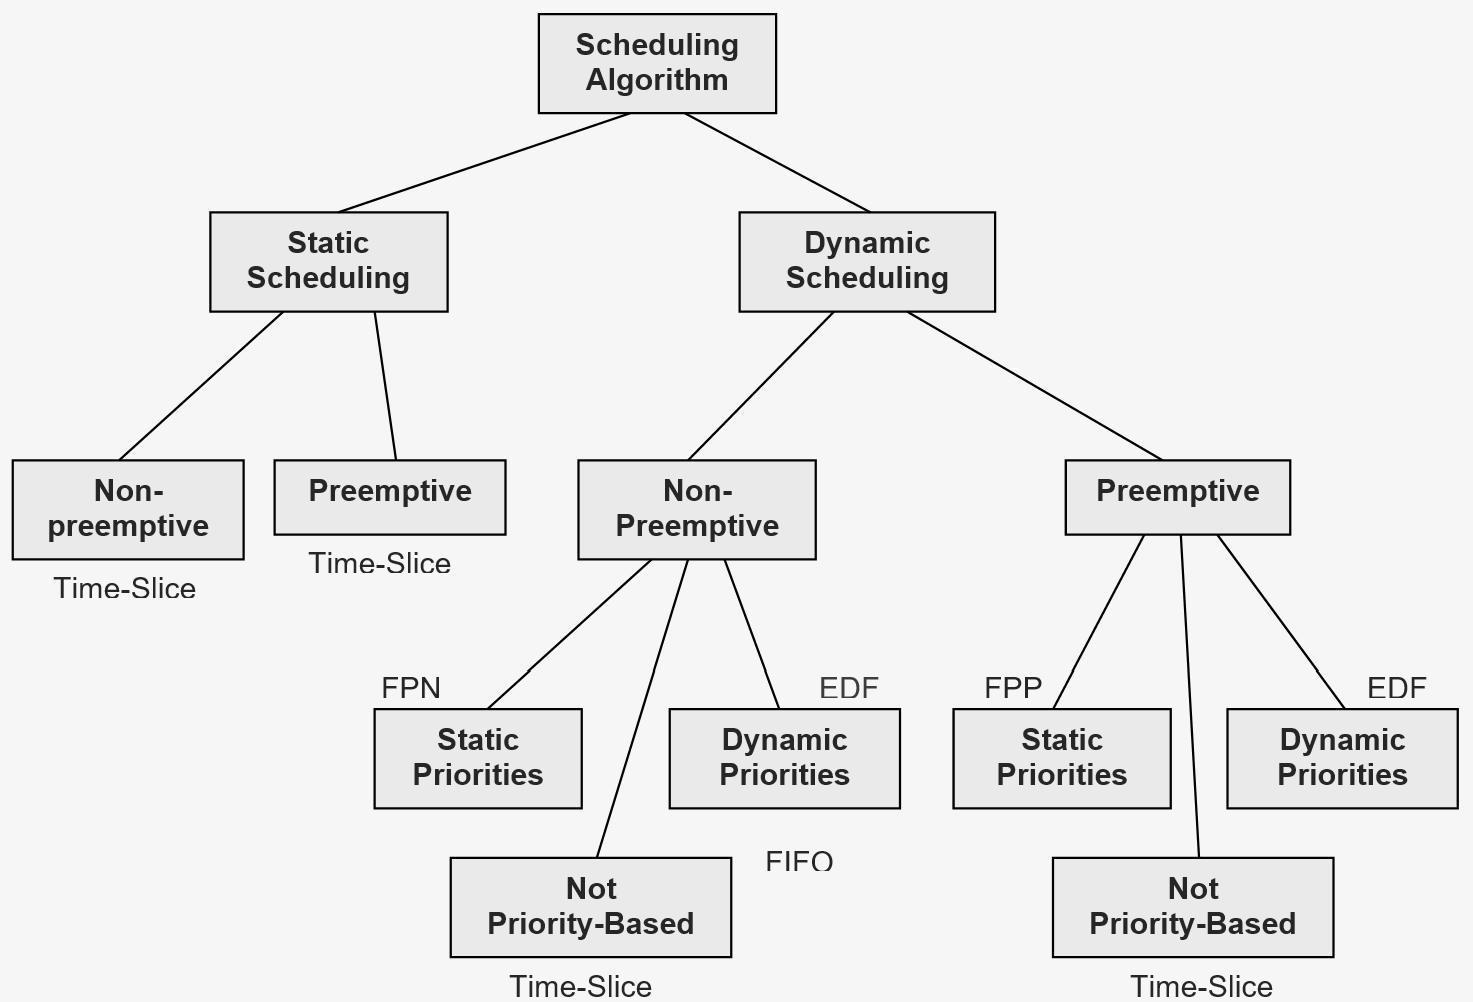
\includegraphics[width=15cm, height=10cm]{Images/image88.png}
    %\caption{}
    \label{fig:Fig 33}
    \end{figure}
\os{\newpage}

{\rot\bf Static Scheduling}\\

Prior to the execution of a taskset an allocation table (dispatching table) with the start times exists, regarding time constraints and dependencies of each task. The dispatcher as part of the RTOS kernel assigns the individual tasks due to this table 

$\rightarrow$ principle of synchronous programming.\\

\textbf{Advantage: }  minimal overhead, as no decisions are needed at runtime. \\

\textbf{Disadvantage: }  restriction to periodic events.\\
\os{\newpage}

{\rot\bf Dynamic Scheduling}\\

Here for the execution of tasks different criteria are used by the dispatcher \textbf{at runtime}, taking into account start times, time conditions (deadlines), and dependencies of each task. Asynchronous programming. Advantage  increased flexibility and the opportunity to respond to aperiodic events. Disadvantage  increased overhead, lower predictability\\

{\rot\bf Static and Dynamic Priorities}\\

(Not to be confused with static/dynamic scheduling). The scheduler can use priorities for the allocation of resources (processor, memory, I/O,{\dots}) to a task. \textbf{Static priorities} are set before running the application and are never changed during runtime. \textbf{Dynamic priorities} can be adjusted for each task \textbf{at runtime}. Furthermore, there are algorithms, using \textbf{No Priorities} at all. 

\subsection{Pre-emption}

Prioritization is an important feature for a scheduler, which describes the capability for displacing a running task for later execution in favour of another task. \\

{\rot\bf{Pre-emptive scheduling }}\\

Pre-emptive scheduling means that a less important task can be displaced by a more important task. The most important task with \textbf{\textit{ready}}-state will be executed immediately. The less important task will be continued again until no other more important task waits with \textbf{\textit{ready}}-state.

	\begin{figure}[h]
    \centering
    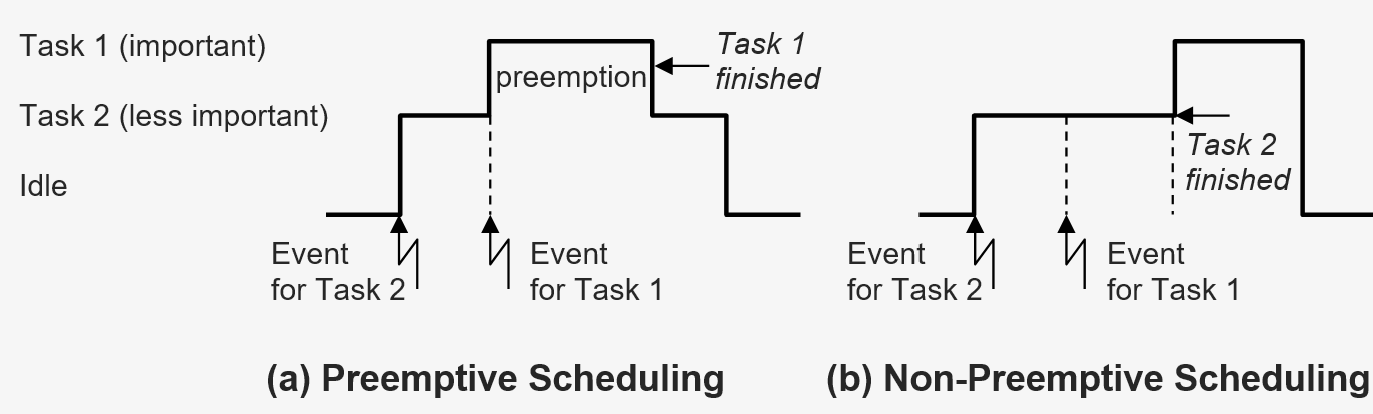
\includegraphics[width=14cm, height=4cm]{Images/image89.png}
    %\caption{}
    \label{fig:Fig 34}
    \end{figure}
\os{\newpage}
{\rot\bf{Non-preemptive scheduling}}\\

Non-preemptive scheduling or co-operative scheduling means, that there is no displacement of a running task. Only after the current task is finished or blocked, the next task with \textbf{\textit{ready}} state is executed.\\

{\rot\bf Time-Slice Scheduling (Round-Robin Scheduling)}\\

Time-Slice Scheduling (time slicing) assigns each task a fixed time slice (Time Slice). The order of task execution corresponds to the sequence of \textbf{\textit{ready}}-tasks entering the task-list of the OS scheduler (FIFO principle). The duration of the time slice for a task can be set individually. This type of time-slice scheduling is a dynamic pre-emptive scheduling. 
\os{\newpage}
\begin{itemize}
	\item TSS does not use priorities
	\item time slot duration can be chosen individually for each task
	\item With time slices chosen fine-grained enough TSS is approaching optimality.
\end{itemize}

	\begin{figure}[h]
    \centering
    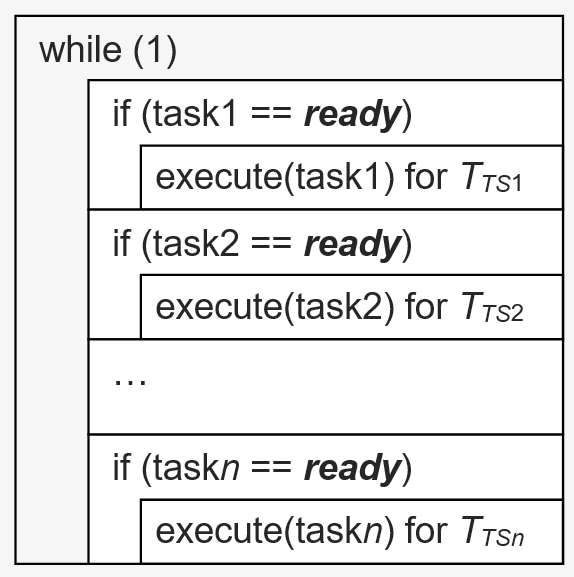
\includegraphics[width=6cm, height=5cm]{Images/image90.png}
    %\caption{}
    \label{fig:Fig 35}
    \end{figure}
\newpage
\textbf{Principle of Time-Slice (Round-Robin) Scheduling: }

\begin{tcolorbox}[colback=blue!5!white,colframe=blue!75!black]
  All \textbf{\textit{ready}}-tasks are queued in a FIFO \\
  Each task \textit{i} gets assigned a time slice (time slice, quantum) \textit{T${}_{TSi}$}
  \begin{itemize}
		\item  the task is preempted, i.e. displaced to the \textbf{\textit{ready}} state
		\item  the task is put at the end of the FIFO queue;
		\item  The first task in the FIFO will be executed.
	\end{itemize}
  
  If a task changes state from \textbf{\textit{blocked}} to \textbf{\textit{ready}}, it will be put at the end of the FIFO queue
\end{tcolorbox}

Typical Applications: \textbf{Kernel-mode programs}. Example: 3 Tasks with $H_{max}$ $<$ 0.778, same as in section 2.2.7:\\
Task T1: period \textit{T}${}_{p1}$ = 10~ms, execution time \textit{T}${}_{e1}$ = 1~ms $\rightarrow$ \textit{H}${}_{1}$ = 0.1\\
Task T2: period \textit{T}${}_{p2}$ = 10~ms, execution time\textit{ T}${}_{e2}$ = 5~ms $\rightarrow$ \textit{H}${}_{2}$ = 0.5\\
Task T3: non-periodic, period \textit{T}${}_{p3}$ = deadline \textit{T}${}_{d3}$ = 15.4~ms, \textit{T}${}_{e3}$ = 2.62~ms $\rightarrow$ \textit{H}${}_{3}$ = 0.17\\


By (2.2) the total CPU utilization \textit{H} = 0.1 + 0.5 + 0.17 = 0.77 \\

One chooses a basic time-slice \textit{T}${}_{TS}$ = 1 ms and assigns individual time slices as multiples of \textit{T}${}_{TS}$ with $\Sigma$\textit{T}${}_{TS}$ = 9 ms:\\

Task T1:    \textit{T}${}_{TS1}$ = 1 $.$\textit{T}${}_{TS}$ = 1 ms $\rightarrow$ \textit{H}${}_{1}$ = \textit{T}${}_{TS1}$/$\Sigma$\textit{T}${}_{TS}$ = 1~ms / 9~ms = 11~\%\\
Task T2:    \textit{T}${}_{TS2}$ = 5 $.$\textit{T}${}_{TS}$ = 5 ms $\rightarrow$ \textit{H}${}_{2}$ = \textit{T}${}_{TS2}$/$\Sigma$\textit{T}${}_{TS}$ = 5~ms / 9~ms = 55~\%\\
Task T3:     \textit{T}${}_{TS3}$ = 3 $.$\textit{T}${}_{TS}$ = 3 ms $\rightarrow$ \textit{H}${}_{3}$ = \textit{T}${}_{TS3}$/$\Sigma$\textit{T}${}_{TS}$ = 3~ms / 9~ms = 33~\%

	\begin{figure}[h]
    \centering
    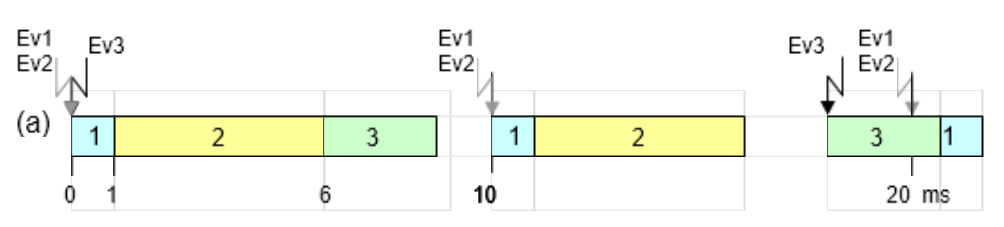
\includegraphics[width=13cm, height=3cm]{Images/image91.png}
    %\caption{}
    \label{fig:Fig 36}
    \end{figure}

In this example the assigned time slices were chosen to be larger than the execution times of each task, in order to avoid preemption. With TSS a context-switch can occur at the end of a time-slice only. which can cause some \textit{jitter} (as with task T1 above).\\

{\rot\bf Fixed Time-Slice-Scheduling }\\

FT scheduling is based on a TDMA approach, requires no priorities, and is therefore frequently used in embedded microcontroller applications without an operating system.\\

A strictly periodic schedule is created with a periodic time \textit{N·T${}_{TS}$}, i.e. with \textit{N} integer multiples of the basic \textit{T${}_{TS}$} time slice. Each task gets assigned one (ore more) basic time slots, large enough to hold the WCET of each:\\

	\begin{figure}[h]
    \centering
    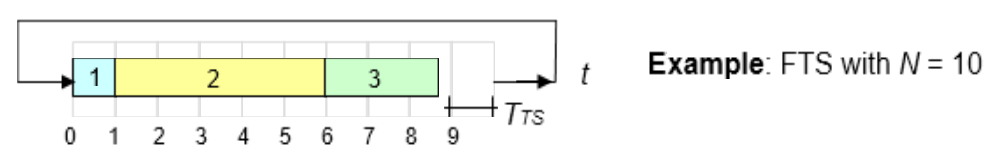
\includegraphics[width=12cm, height=2cm]{Images/image92.png}
    %\caption{}
    \label{fig:Fig 37}
    \end{figure}

Conditions for Events are polled within each task, if a task is not finished at the end of its timeslice, it can be preempted (\textbf{\textit{preemptive FTS}})or not (\textbf{\textit{cooperative FTS}}).\\
\os{\newpage}

The previous example with three tasks, and an idle task T4 at a period \textit{N}$\mathrm{\bullet}$\textit{T${}_{TS}$} = $\Sigma$\textit{T${}_{TS}$} = 10 ms is realized, the time slices are chosen as multiples of \textit{T${}_{TS}$} = 1 ms as follows \\

Task T1:    \textit{T${}_{TS}$}${}_{1}$ = 1 $.$\textit{T${}_{TS}$} = 1 ms $\rightarrow$ \textit{H}${}_{1}$ = \textit{T${}_{TS}$}${}_{1}$/$\Sigma$\textit{T${}_{TS}$} = 1~ms / 10~ms = 10~\%
Task T2:    \textit{T${}_{TS}$}${}_{2}$ = 5 $.$\textit{T${}_{TS}$} = 5 ms $\rightarrow$ \textit{H}${}_{2}$ = \textit{T${}_{TS}$}${}_{2}$/$\Sigma$\textit{T${}_{TS}$} = 5~ms / 10~ms = 50~\%
Task T3:     \textit{T${}_{TS}$}${}_{3}$ = 3 $.$\textit{T${}_{TS}$} = 3 ms $\rightarrow$ \textit{H}${}_{3}$ = \textit{T${}_{TS}$}${}_{3}$/2$\Sigma$\textit{T${}_{TS}$} = 3~ms / 10~ms = 30~\%
Task T4 (idle) \textit{T${}_{TS}$}${}_{4}$ = 1 $.$\textit{T${}_{TS}$} = 1 ms $\rightarrow$ \textit{H}${}_{4}$ = 10~\%

	\begin{figure}[h]
    \centering
    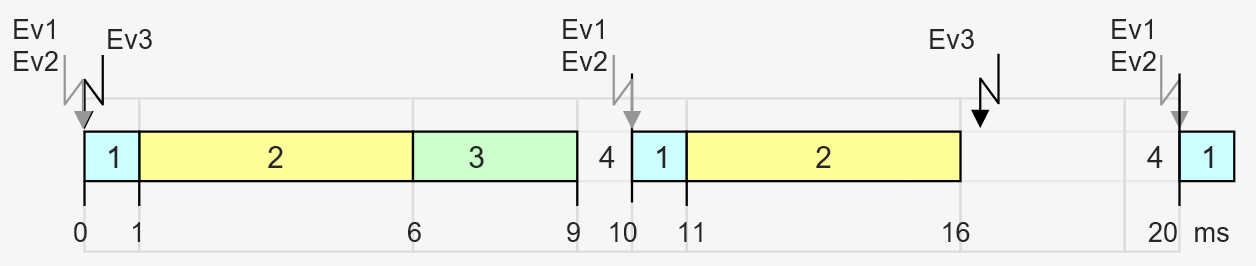
\includegraphics[width=13cm, height=3cm]{Images/image93.png}
    %\caption{}
    \label{fig:Fig 38}
    \end{figure}

T3 runs for the second time at \textit{t} = 26 ms the delay of 10 ms does not result in a T3-deadline violation. The idle task T4 provides a placeholder for unused CPU load, which can be used in modern CPUs for power saving features.\\

\textbf{Advantage of fixed TSS}: the execution times can be defined exactly!\\

{\rot\bf Binary Fixed Time-Slice-Scheduling }\\

If task periodic times \textit{T${}_{Pi}$} can be represented as power-of-2 integer multiples of a basic time slice \textit{T${}_{TS}$}, one can obtain a periodic binary schedule:\\

	\begin{figure}[h]
    \centering
    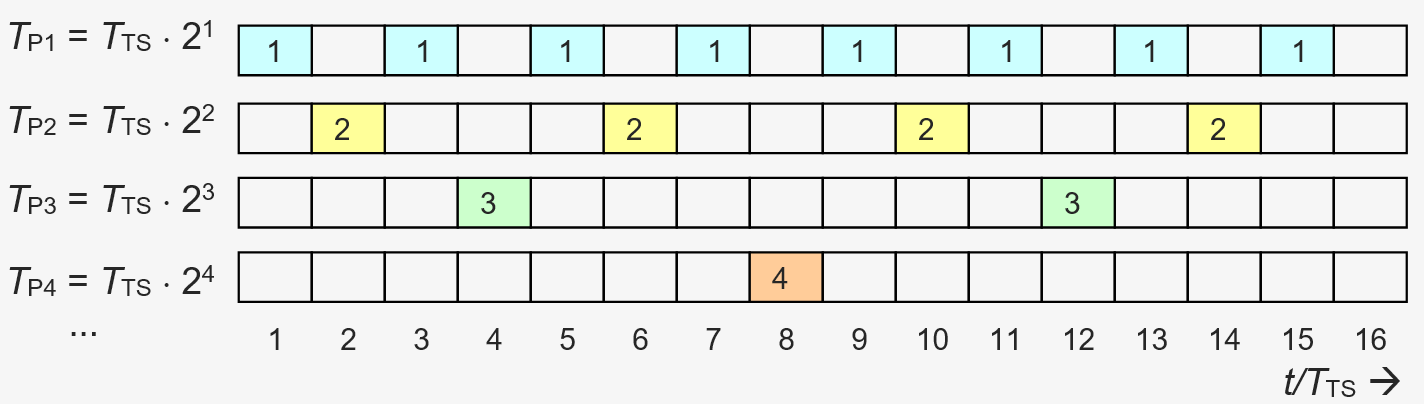
\includegraphics[width=12cm, height=3.5cm]{Images/image94.png}
    %\caption{}
    \label{fig:Fig 39}
    \end{figure}

If the maximum time of execution is \textit{T}${}_{TS}$ and equal for each task, the utilization for each task is 

\begin{equation}
	 H_{i} =\frac{T_{ei} }{T_{pi} } =\frac{T_{TS} }{2^{i} \cdot T_{TS} } =2^{-i} \hspace{3cm} \sum_{i=1}^N H_{i} \stackrel{N\to \infty }{\longrightarrow} 1
\label{EQ }
\end{equation}

Thus, the fastest task with periodic time \textit{T${}_{p}$}${}_{1}$ = 2$.$\textit{T}${}_{TS}$ is assigned 50~\% of the complete processing time, task 2 with periodic time \textit{T${}_{p}$}${}_{2}$ = 4$.$\textit{T}${}_{TS}$ gets assigned 25~\%, task 3 gets 12.5~\%, {\dots}\\

From (2.3) it shows, that the total utilization of \textit{H} aiming with an infinite number of tasks to 100\%, thus, there will be no overload situations, if all tasks meet their maximum execution time \textit{T${}_{TS}$} requirement (easily guaranteed with a preemptive schedule).\\

\textit{   T${}_{TS}$} $\mathrm{\ge}$ max(\textit{T${}_{e}$}${}_{1}$,\textit{ T${}_{e}$}${}_{2}$,\textit{ T${}_{e}$}${}_{3}$, ..)\\

With a non-preemptive schedule (cooperative task schedule) maximum execution times \textit{T${}_{ei}$} have to be determined carefully (WCET determination), such, that each task can complete execution within the basic \textit{T${}_{TS}$}. If a task gets delayed for some reasons (like high priority interrupts during execution) the complete schedule will get delayed.\\
\os{\newpage}
\nsl{\newpage}

\textbf{Advantages }\\

Binary fixed time-slice scheduling is

\begin{itemize}
	\item  quite suitable with multirate sampling systems (e.g. oversampling, when integer multiples of a common sampling frequency are needed).
	\item  a very simple scheduling without priorities,
	\item  suitable in a non-preemptive realization for even small microcontrollers without OS. 
	\item  Time and duration of execution for each task is guaranteed (apart from interrupts)
\end{itemize}

\textbf{Disadvantages }

\begin{itemize}
	\item \textbf{ }Binary time-slice scheduling is not fully flexible with arbitrary periodic times and execution times
	\item  can turn into very complex software, especially with integrating tasks with execution time larger than \textit{T${}_{TS}$}.
\end{itemize}
\os{\newpage}
\textbf{Lab-Experiment}   \textbf{\underbar{AVR-Timer-Interrupts-(FTS-Scheduling)}}

	\begin{figure}[h]
    \centering
    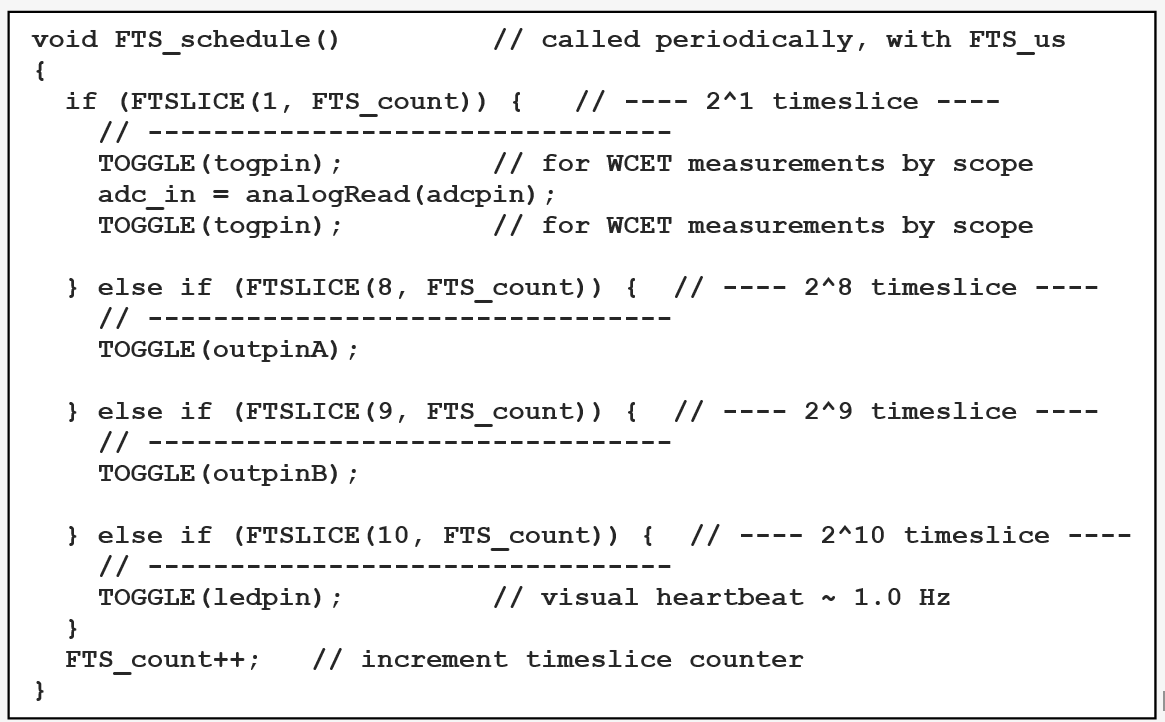
\includegraphics[width=13cm, height=7cm]{Images/image95.png}
    %\caption{}
    \label{fig:Fig 40}
    \end{figure}

\textbf{\underbar{Sketch for Arduino Nano}  (FixedTimeSlice.ino)}\\
\newpage
\textbf{Example}: 4 periodic tasks (on an AVR $\mu$C, from section Digital PID Control with 4 Tasks) \\

\textit{T${}_{p}$}${}_{1}$ = \textit{T${}_{p}$}${}_{2}$ = 1 ms, \textit{T${}_{p}$}${}_{3}$ = 16 ms, \textit{T${}_{p}$}${}_{4}$ = 8 ms

\textit{T${}_{e}$}${}_{1}$ = 50 $\mu$s, \textit{T${}_{e}$}${}_{2}$ = 0.3 ms, \textit{T${}_{p}$}${}_{3}$ = 40 $\mu$s, \textit{T${}_{p}$}${}_{4}$ = 40 $\mu$s

\textit{H}${}_{1}$ = 5 \%, \textit{H}${}_{2}$ = 30 \%, \textit{H}${}_{3}$ = 0.1/20 = 0.5 \%, $\rightarrow$ \textit{H}${}_{4}$ = 0.05/20 = 0.25 \%  \textit{H} = 30.75 \%\\

Solution with Binary time-slice schedule with 3 Tasks, \textit{T${}_{TS}$} = 0.5 ms, \textit{T${}_{TS}$} $\mathrm{\ge}$ max(\textit{T${}_{ei}$}) = max(0.3, 0.05, 0.005 0.0025 ms) tasks with the same periodic times run in the same time-slice:\\

$\rightarrow$ T1 und T2 executed successively in the 2 Timeslice 2·\textit{T${}_{TS}$ }= 1 ms\\
 
  	\os{\begin{figure}[h]
    \centering
    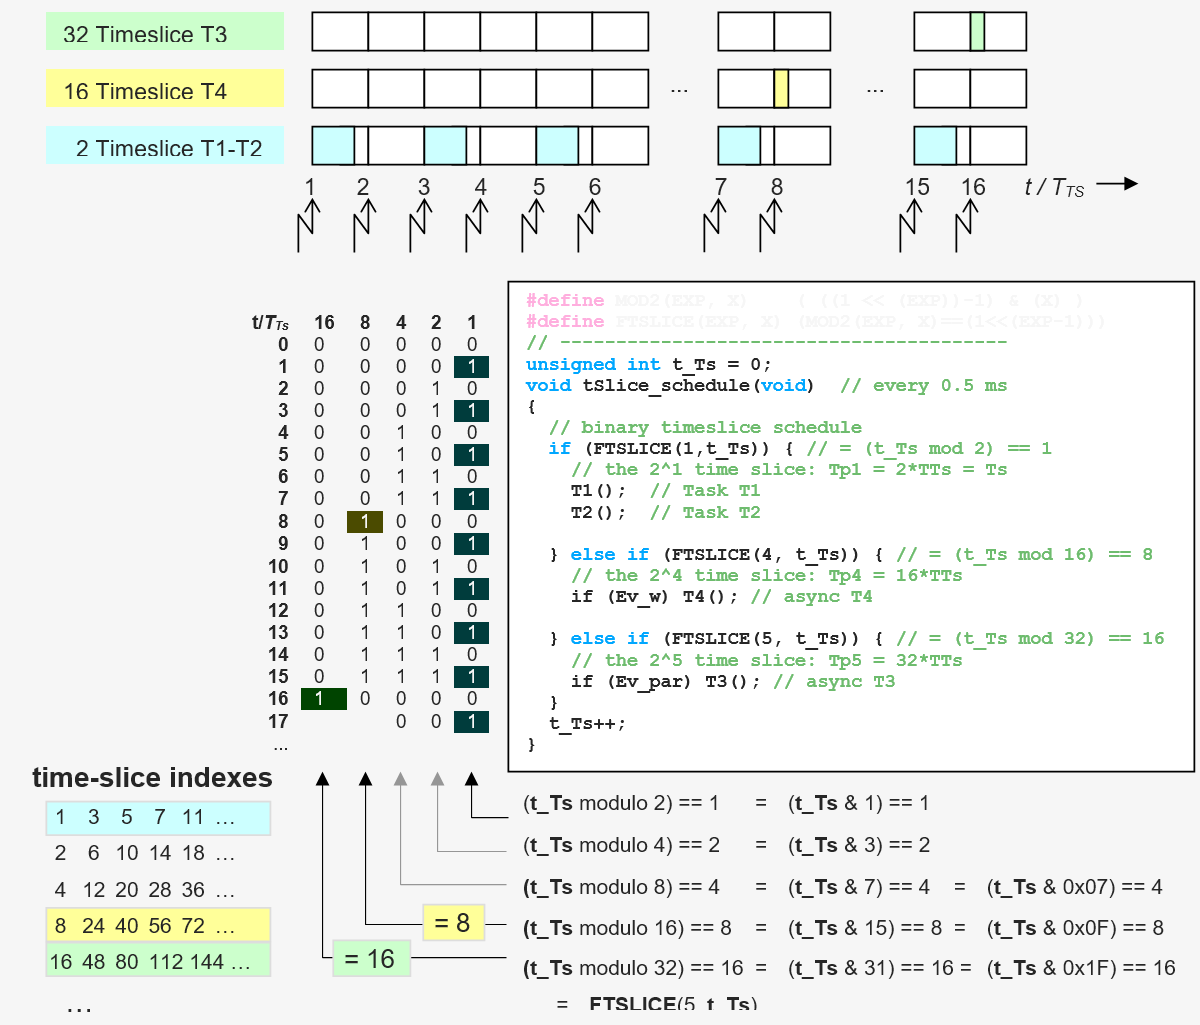
\includegraphics[width=15cm, height=10.8cm]{Images/image96.png}
    %\caption{}
    \label{fig:Fig 41}
    \end{figure}}
    
 	\nsl{\begin{figure}[h]
    \centering
    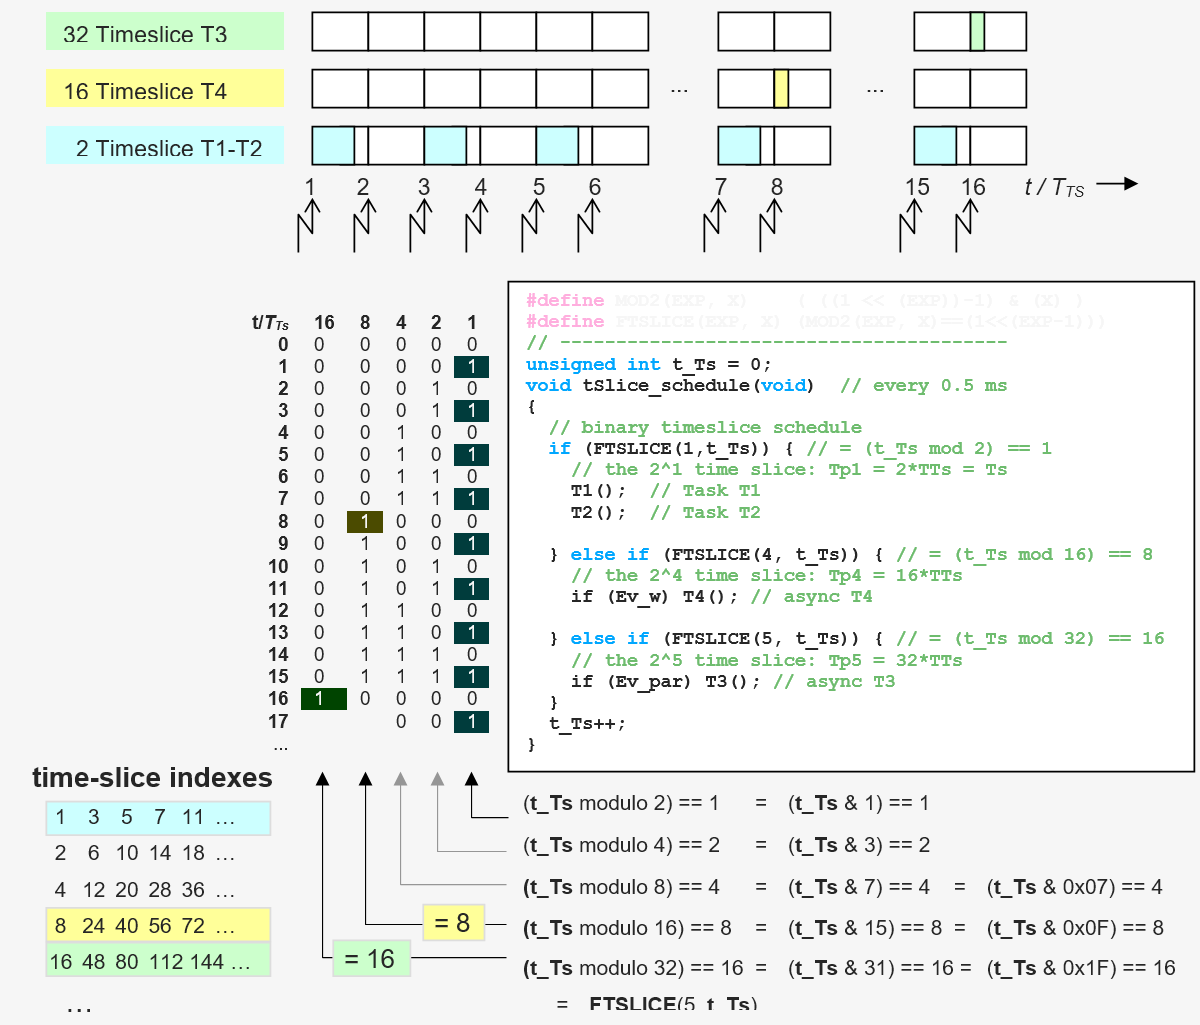
\includegraphics[width=15cm, height=11cm]{Images/image96.png}
    %\caption{}
    \label{fig:Fig 41}
    \end{figure}}
\os{\newpage}

Proof for collision-free assignment of time-slice indexes  (with \textit{k},\textit{l} $\in$ \textbf{$\boldsymbol{\mathbb{Z}}$}  integers). For some period \textit{N} we get time slices at indexes  \textit{n${}_{k}$}  =  \textit{k$\bullet$N  +  $\frac{N}{2} $}  e.g.: 2, 6, 10, 14, ..\\

thus, for period 2\textit{N} (next time slice) we get    \textit{m${}_{l}$} =  \textit{l$\bullet$}2\textit{N  +  N  }e.g.: 4, 12, 20, 28, ..\\

for a collision, we set \textit{n${}_{k}$} ${\mathop{=}\limits^{!}} $ \textit{m${}_{l}$}. Division by \textit{N} on both sides shows \textit{k} + 0.5 ${\mathop{=}\limits^{!}} $ 2$\mathrm{\bullet}$\textit{l} + 1, which has no solution with integers \textit{k} and \textit{l}, thus the above assignment is without any conflict all time slice indexes (proof by full induction) !\\
\newpage

{\rot\bf FIFO Scheduling}\\

The name derives from the FIFO (first in, first out) principle of a waiting queue.

 	\begin{figure}[h]
    \centering
    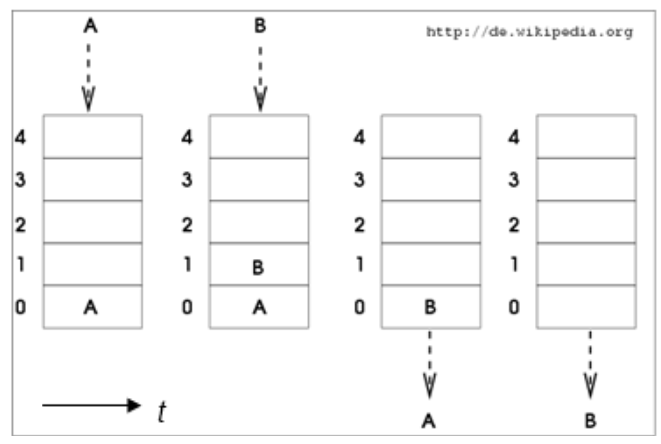
\includegraphics[width=9cm, height=4cm]{Images/image97.png}
    %\caption{}
    \label{fig:Fig 42}
    \end{figure}

where elements put into a queue in a certain order of sequence, are taken out in the same order of sequence.With a \textbf{FIFO scheduler}, the tasks are processed in the same order in which they have taken the ready state. An running task is not interrupted, it is a \textbf{non-preemptive}, \textbf{dynamic} scheduler.\\

\textbf{Advantage:}   Very simple implementation, sometimes used in universal OS\\
\textbf{Disadvantage:}  Bad real-time performance, violations of time conditions even at low processing demands\\

\textbf{Example}: Two tasks with FIFO scheduling

Task 1: \textit{T}${}_{p1}$ = 150 ms, \textit{T}${}_{e1}$ = 15 ms   \textit{H}${}_{1}$ = 0.1

Task 2: \textit{T}${}_{p2}$ = 10 ms,  \textit{T}${}_{e2}$ = 1 ms    \textit{H}${}_{2}$ = 0.1

For both periodic tasks there is a time bound (deadline) with the next period. With (2.2) 

\textit{H} = \textit{H}${}_{1}$ + \textit{H}${}_{2}$ = 0.1 + 0.1 = 0.2 

For 20 \% processor demand only, it should be easy to find a schedule for this taskset, but:

 	\begin{figure}[h]
    \centering
    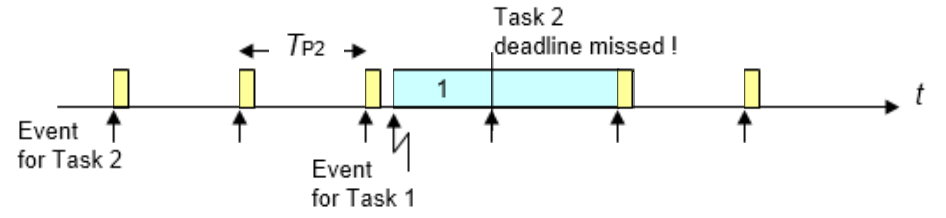
\includegraphics[width=12cm, height=2.5cm]{Images/image98.png}
    %\caption{}
    \label{fig:Fig 43}
    \end{figure}

This simple example shows that even at a very low processor demand, a FIFO scheduler \textbf{cannot} \textbf{guarantee} compliance with the real-time conditions.\\

{\rot\bf Fixed-Priority Scheduling}\\

For fixed-priority scheduling, each task is assigned a fixed priority. The ready task with the highest priority waiting in the scheduler's queue is assigned to the processor. Fixed-priority scheduling is dynamic scheduling with static priorities. (often used with interrupt processing of microprocessors, pre-emptive or non-preemptive).

\begin{enumerate}
	\item  \textbf{Fixed-Priority-Preemptive Scheduling (FPP)}\\
	If a task with higher priority than the currently running gets into the ready state, then the current task is interrupted (displaced, preempted) and the task with the higher priority is assigned to the processor immediately.
	
	\item  \textbf{Fixed-Priority-Non-Preemptive Scheduling (FPN)}\\
	If a task with higher priority than the currently running gets into the ready state, then the task is assigned to the processor only after the current task is either completed or blocked.
\end{enumerate}

\textbf{Advantage}: with FPP, the compliance with the real-time conditions can be guaranteed (unlike to FIFO scheduling), if the priorities were assigned appropriate. \\

\nsl{The assignment of priorities to tasks is an important step in the development of a real-time application.\\}

{\rot\bf Rate-Monotonic-Scheduling (RMS)}\\

For purely periodic applications, there is a rule, the so-called \textbf{rate-monotonic scheduling rule}, which states, that the priority of the tasks to be performed is inversely proportional to their periodic time

\begin{equation}
	PR_{i} \sim \frac{1}{T_{pi} } 
\label{EQ }
\end{equation}

$PR_i$ Priority task i, $T_{pi}$ Periodic time of task i under the (rather idealized) conditions:

\begin{itemize}
	\item  Pre-emptive scheduling is used
	\item  The periodic times \textit{T${}_{Pi}$} are constant 		
	\item  The time limits (deadlines) are equal to the periodic times \textit{T${}_{Pi}$}
	\item  The execution times are known and constant \textit{T${}_{ei}$}
	\item  The tasks are independent from each other (can not deadlock)
\end{itemize}

\textbf{Example}: (same as with FIFO scheduling in section 2.2.6). Two tasks with Fixed-Priority-Preemptive Scheduling (FPP):\\

Task 1: \textit{T}${}_{p1}$ = 150 ms, \textit{T}${}_{e1}$ = 15 ms,   lower priority by   (2.4)\\
Task 2: \textit{T}${}_{p2}$ = 10 ms,  \textit{T}${}_{e2}$ = 1 ms   higher priority by (2.4)\\

 	\begin{figure}[h]
    \centering
    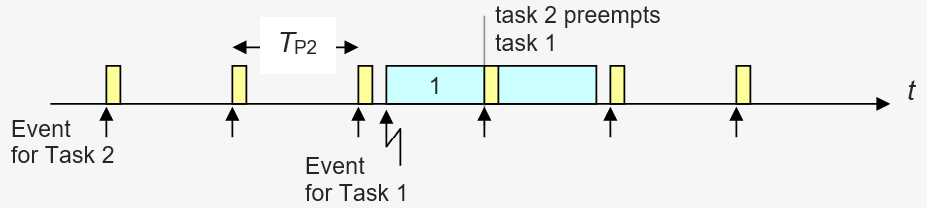
\includegraphics[width=12cm, height=2.5cm]{Images/image99.png}
    %\caption{}
    \label{fig:Fig 44}
    \end{figure}

The running task 1 is displaced with an event for task 2, which has higher priority (its state goes from \textbf{\textit{blocked}}  \textbf{\textit{ready}}), so that the deadline of task 2 is not violated (in contrast to FIFO scheduling).\\

Obviously,\textbf{ FPP scheduling} with \textbf{RMS} provides much better results than FIFO scheduling. In contrast, with \textbf{FPN}, the deadlines of task 2 would be violated !. In general\\

\begin{tcolorbox}[colback=blue!5!white,colframe=blue!75!black]
 	With periodic tasks with fixed priorities and deadlines equal to their periodic times, rate-monotonic scheduling (RMS) provides for an optimal priority allocation.
\end{tcolorbox}

This also means that FPP scheduling with RMS always delivers an executable schedule, if one exists. However, the overall CPU utilization may not exceed \textit{H${}_{max}$ }([1], by Liu)\\

\begin{equation}
	H_{\max } =n\cdot \left(2^{1/n} -1\right)=n\cdot \left(\sqrt[{n}]{2} -1\right) 
\label{EQ }
\end{equation}

$n$ number of tasks\\

\begin{table}[h!]
\setlength{\tabcolsep}{10pt} % Default value: 6pt
\renewcommand{\arraystretch}{1.5} % Default value: 1
\small
\centering
 \begin{tabular}{|c|c|c|c|} 
 \hline
 \textbf{n} & \textbf{$H_{max}$} \\ [0.1ex] \hline
1 & 1.000000 \\ \hline
2 & 0.828427 \\ \hline
3 & 0.779763 \\  \hline
4 & 0.756828 \\ \hline
5 & 0.743492 \\ \hline
10 & 0.717735 \\ \hline 
20 & 0.705298 \\ \hline 
50 & 0.697974 \\ \hline 
100 & 0.695555 \\ \hline 
1000 & 0.693387 \\ \hline 
10000 & 0.693171 \\ \hline 
 \end{tabular}
 %\caption{\textbf{}}
 \label{}
\end{table}

The limit (2.5) can be used to examine the feasibility of a (periodic) taskset and to guarantee the conformance with all time limits.FPP with RMS is very popular because of its simplicity. \\

However, there are problems at very high utilization (beyond or near \textit{H${}_{max}$}) and with RMS at the same or nearly the same time periods, delivering same task priorities. Furthermore, there are sometimes difficulties in approaching non-periodic processes by periodic processes with sufficient precision.\\

\os{\newpage}
\textbf{Example 1:} 3 Tasks with \textit{H}${}_{max}$ $\mathrm{>}$ 0.778, from [W\"{o}rnB] : \\
Task T1: period \textit{T}${}_{p1}$ = 10~ms, execution time \textit{T}${}_{e1}$ = 1~ms $\rightarrow$ \textit{H}${}_{1}$ = 0.1\\
Task T2: period \textit{T}${}_{p2}$ = 10~ms, execution time\textit{ T}${}_{e2}$ = 5~ms $\rightarrow$ \textit{H}${}_{2}$ = 0.5\\
Task T3: non-periodic, deadline = \textit{T}${}_{d3}$ = 15.4~ms, execution time\textit{ T}${}_{e3}$ = 5.5~ms\\

By (2.2) the total CPU utilization \textit{H} = 0.1 + 0.5 + 0.357 = 0.957, amost 100 \% !But with (2.5) \textit{H} $\mathrm{>}$ \textit{H}${}_{max}$ $\mathrm{>}$ 0.78 deadlines will be violated with \textbf{FPP/RMS} with 3 tasks. FPP/RMS \textbf{can't deliver an executable schedule}, as this example shows:\\

By (2.4) one has 2 choices for assigning the priorities due to the equal periods \textit{T}${}_{p1}$\textit{ }and \textit{T}${}_{p2}$:\\

\begin{table}[h!]
\setlength{\tabcolsep}{10pt} % Default value: 6pt
\renewcommand{\arraystretch}{1.5} % Default value: 1
\small
\centering
 \begin{tabular}{|c|c|c|c|} 
 \hline
 \textbf{Priority assignment (a)} & \textbf{Priority assignment (b)} \\ [0.1ex] 
 \hline
 T1  high priority & T2  high  priority \\ 
 \hline
 T2  medium priority & T1  medium priority \\ 
  \hline
 T3  low priority & T3  low priority  \\ 
 \hline
 \end{tabular}
 %\caption{\textbf{}}
 %\label{Intrinsic}
\end{table}
\os{\newpage}
In both cases there is a violation of the T3 deadline, if all tasks get \textbf{\textit{ready}} the same time at \textit{t} = 0: 

 	\begin{figure}[h]
    \centering
    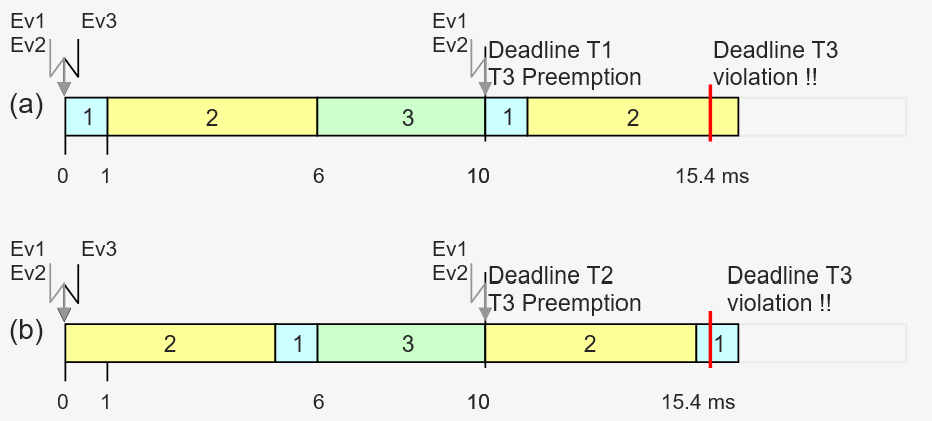
\includegraphics[width=12cm, height=5cm]{Images/image100.png}
    %\caption{}
    \label{fig:Fig 45}
    \end{figure}

{\nsl{\newpage}}
Of course, the violation of T3 deadline in the example above occurs due to the deliberate disregard of the load limit \textit{H${}_{max}$}, by \eqref{fig:Fig 45}. If one meets the max. load requirement \textit{H} $\mathrm{<}$ 78\% (n = 3), there is violation of the T3 deadline.\\

However, with growing number of tasks the maximum load goes down as low as 70\% (from n $\mathrm{>}$ 10), which is surprisingly low. Ideas to achieve higher processor loads lead to dynamic assignment of priorities.\\

\textbf{Example 2:} 3 Tasks with \textit{H}${}_{max}$ $\mathrm{<}$ 0.778, from [W\"{o}rnB] :\\
Task T1: period \textit{T}${}_{p1}$ = 10~ms, execution time \textit{T}${}_{e1}$ = 1~ms  $\rightarrow$ \textit{H}${}_{1}$ = 0.1\\
Task T2: period \textit{T}${}_{p2}$ = 10~ms, execution time\textit{ T}${}_{e2}$ = 5~ms  $\rightarrow$ \textit{H}${}_{2}$ = 0.5\\
Task T3: non-periodic, period \textit{T}${}_{p3}$ = deadline \textit{T}${}_{d3}$ = 15.4~ms, \textit{T}${}_{e3}$ = 2.62~ms  $\rightarrow$ \textit{H}${}_{3}$ = 0.17\\

By (2.2) the total CPU utilization \textit{H} = 0.1 + 0.5 + 0.17 = 0.77 With (2.5) \textit{H} $\mathrm{<}$ \textit{H}${}_{max}$ = 0.78 deadlines will be not violated with FPP/RMS with 3 tasks:\\

By (2.4) one has 2 choices for assigning the priorities due to the equal periods \textit{T}${}_{p1}$\textit{ }and \textit{T}${}_{p2}$:

\begin{table}[h!]
\setlength{\tabcolsep}{10pt} % Default value: 6pt
\renewcommand{\arraystretch}{1.5} % Default value: 1
\small
\centering
 \begin{tabular}{|c|c|c|c|} 
 \hline
 \textbf{Priority assignment (a)} & \textbf{Priority assignment (b)} \\ [0.1ex] 
 \hline
 T1  high priority & T2  high  priority \\ 
 \hline
 T2  medium priority & T1  medium priority \\ 
  \hline
 T3  low priority & T3  low priority  \\ 
 \hline
 \end{tabular}
 %\caption{\textbf{}}
 %\label{Intrinsic}
\end{table}

In both cases there is no violation of the T3 deadline, even if all tasks get \textbf{\textit{ready}} the same time at \textit{t} = 0: 
	
	\begin{figure}[h]
    \centering
    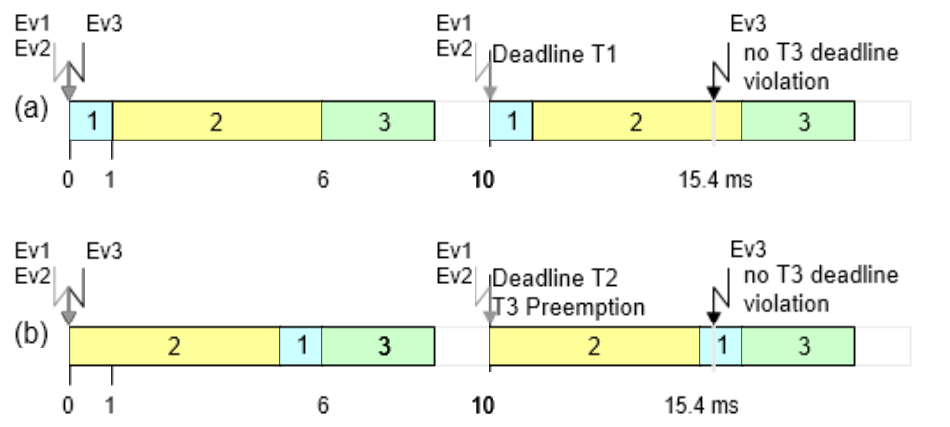
\includegraphics[width=12cm, height=5cm]{Images/image187.png}
    %\caption{}
    \label{fig:Fig 46}
    \end{figure}
\nsl{\newpage}
$\rightarrow$ If one meets the max. load requirement \textit{H} $\mathrm{<}$ 78\% (n = 3), there is violation of the T3 deadline.\\

However, with 3 tasks the maximum load allowed is as low as 77.8\% (for \textit{n} = 3), which is surprisingly low.\\

Ideas to achieve higher processor loads lead to dynamic assignment of priorities \\
$\rightarrow$ next sections.\\
\os{\newpage}

{\rot\bf Earliest-Deadline-First Scheduling (EDF)}\\

In Earliest-Deadline-First Scheduling (EDF) the Task Processor is granted to that \textbf{\textit{ready}}-task, which is closest to its time limit (deadline). This is achieved by assigning the task priorities according to the vicinity to the individual deadlines. EDF is dynamic scheduling with dynamic priorities, either preemptive or non-preemptive\\

For \textbf{preemptive EDF scheduling} a context-switch is made, when a task with earlier time bound gets \textbf{\textit{ready}}. In \textbf{non-preemptive EDF scheduling} is the task with the shortest time interval ist executed only, if the currently running task is finished or blocked.\\

Pre-emptive EDF scheduling, is used more frequently than non-preemptive EDF scheduling, which is essentially only used when non-interruptible processes are to be managed, such as disk access.\\

\textbf{Advantage}: With pre-emptive EDF scheduling 100 \% CPU utilization can be achieved. \\

\textbf{Example} with 3 Tasks (same as in section 2.2.7): Task T1: period \textit{T}${}_{p1}$ = 10~ms, execution time \textit{T}${}_{e1}$ = 1~ms  \textit{H}${}_{1}$ = 0.1Task T2: period \textit{T}${}_{p2}$ = 10~ms, execution time\textit{ T}${}_{e2}$ = 5~ms  \textit{H}${}_{2}$ = 0.5Task T3: non-periodic, deadline = \textit{T}${}_{d3}$ = 15.4~ms, execution time\textit{ T}${}_{e3}$ = 5.5~ms(each periodic time is assumed to be deadline). Again, by (2.2) the total CPU utilization \textit{H} = 0.1 + 0.5 + 0.357 = 0.957, almost 100 \% !\\

 	\begin{figure}[h]
    \centering
    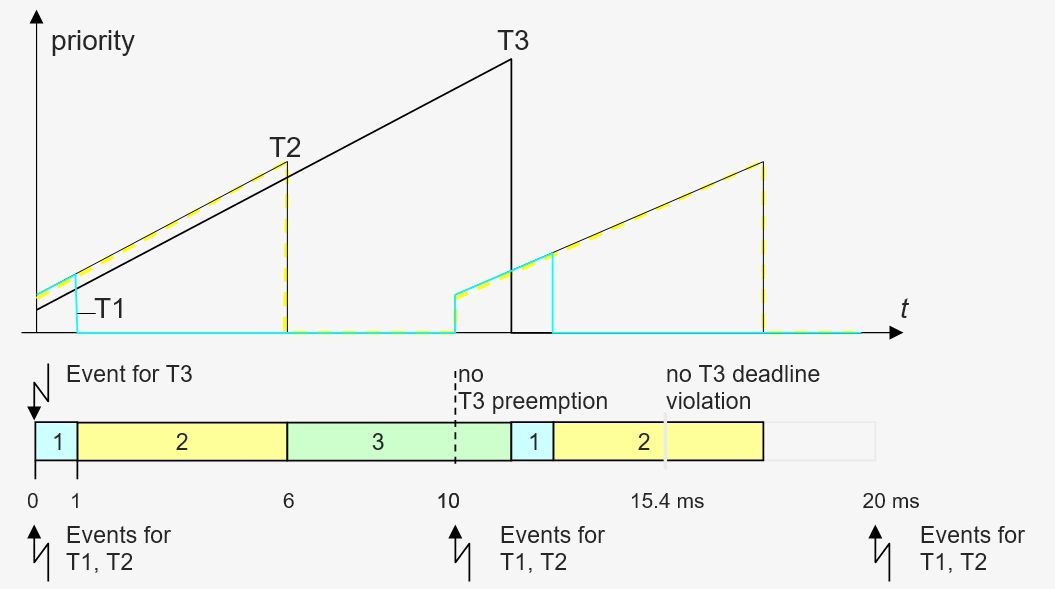
\includegraphics[width=13cm, height=5.5cm]{Images/image101.png}
    %\caption{}
    \label{fig:Fig 47}
    \end{figure}


(at \textit{t} = 0, T1 and T2 have equal priorities, due to equal deadlines, in such a case, the scheduler decides randomly, e.g. for the task with the lower id).\\

It can be seen, that with EDF scheduling an executable schedule is found. Liu [W\"{o}rnB] shows, that EDF scheduling is an optimal scheduling with

\begin{equation}
	H \mathrm{<} 100 \% for\ preemptive\ EDF\ scheduling
\label{EQ }
\end{equation}

\textbf{Advantage}: 

\begin{enumerate}
\item  As long as the processor utilization is less than 100 \% with a uniprocessor system, EDF  scheduling delivers an executable schedule and compliance with all time conditions is guaranteed.
\end{enumerate}

\textbf{Disadvantages:}

\begin{enumerate}
\item Increased computational complexity for the dynamic priorities needed at run time.

\item The sequence of task assignment is difficult to control.

\item The time of execution is difficult to control with fixed time requirements.
\end{enumerate}
\newpage

\section{Task-Synchronization and Communication}

As most of the resources may only be used exclusively, tasks that request these resources must be synchronized for exclusive use, sometimes with regard to some sequence of access. \\

Thus, the OS provides \textbf{means for} \textbf{synchronization} either for 

\begin{enumerate}
\item  Mutual exclusion, and 
\item  Co-operation (sequence of access).
\end{enumerate}
\os{\newpage}
{\rot\bf Synchronization }\\

The problem of synchronization of tasks arises when these tasks are not independent from each other. Dependencies arise, when common resources are be used, then the access needs to be coordinated. Common resources may be

\begin{enumerate}
	\item  \textbf{Data: }Multiple tasks read and write access to shared variable, like tables. (without synchronization, uncoordinated access could result in inconsistent data, e.g. when task 1 is reading values of a table, while another task 2 is updating that table partly.

	\item  \textbf{Devices: } Multiple tasks using common devices such as sensors or actuators. (again, coordination is necessary to not to send e.g. contradictional commands of two tasks to a stepper motor drive).

	\item  \textbf{Programs: } Several tasks share common programs, such as device drivers. Competing calls to a device driver must be assured to leave consistent application states.
\end{enumerate}
\os{\newpage}
\textbf{ Example}: Two tasks compete for access to a data table:\\

Task 1 is reading several temperature sensors, and stores these values in a table\\
Task 2 is reading this table, and prints out the temperature distribution.\\

Without synchronization, this can lead to erroneous results if, for example task 1, the common table has not yet been fully updated, while task 2 accesses. Then, task 2 gets mixed new and old temperature values, which can lead to undefined states !

 	\begin{figure}[h]
    \centering
    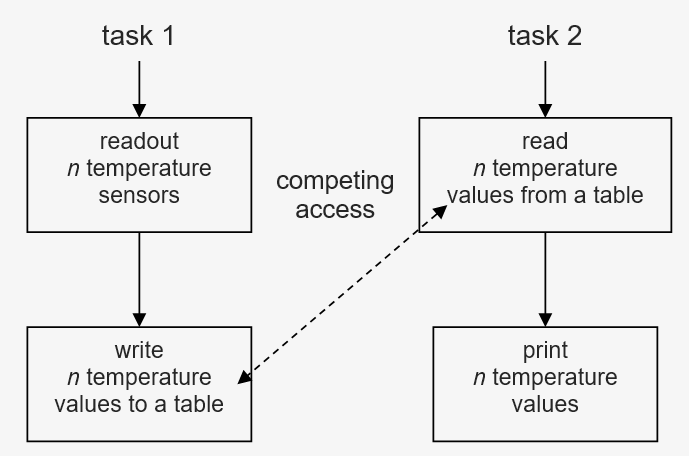
\includegraphics[width=9cm, height=6cm]{Images/image102.png}
    %\caption{}
    \label{fig:Fig 48}
    \end{figure}

\newpage  
There are two basic types of synchronization:

\begin{enumerate}
\item The \textbf{Mutual Exclusion }or shortly called \textbf{\textit{Mutex}}, ensures that access to a common resource is permitted only to one task at a time. 

 	\begin{figure}[h]
    \centering
    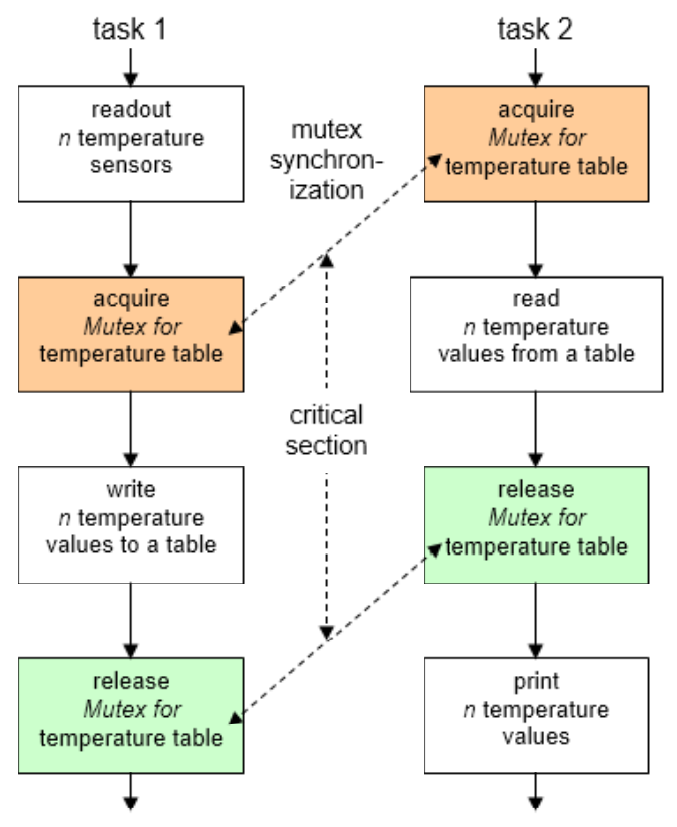
\includegraphics[width=9cm, height=9cm]{Images/image103.png}
    %\caption{}
    \label{fig:Fig 49}
    \end{figure}
\os{\newpage}
\textbf{Example:} of temperature measurement using the \textbf{mutex} synchronization.\\

For the protection of the common temperature table, a \textbf{mutex} is defined, toexclude the possibility that both tasks \textbf{access} this resource simultaneously.Before entering the critical section a task tries to acquire the mutex from the OS. If the mutex is already occupied by the other task, the newly accessing task is blocked\textbf{\textit{ }}until the other task \textbf{releases} the \textbf{mutex} again. The task will \textbf{un-block,} acquisition of the \textbf{mutex} succeeds, allowing the task to enter the critical section. The sequence, which task 1 or 2 acquires the \textbf{mutex} does not matter.

\item Synchronization, where the order of access to common resources matters is called \textbf{cooperation} --unlike as with\textbf{ mutex synchronization}, which doesn't regard the order of task requests.

 	\begin{figure}[h]
    \centering
    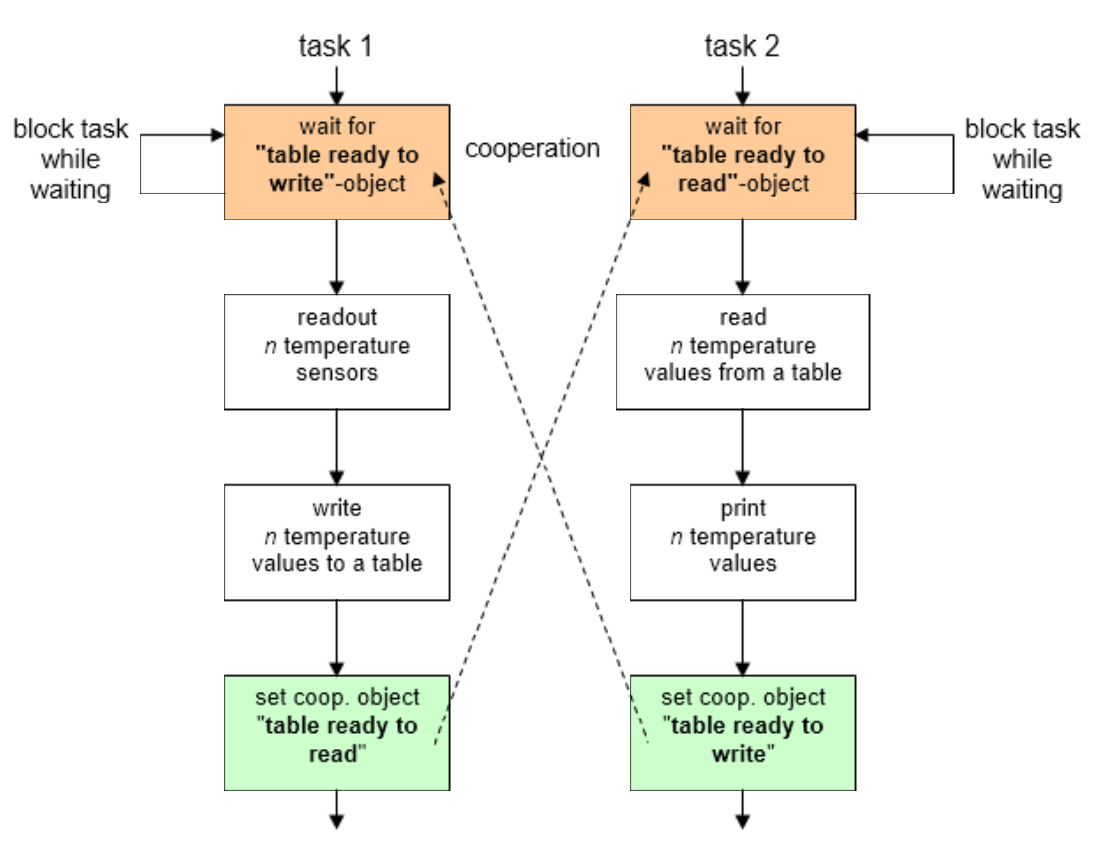
\includegraphics[width=14cm, height=10cm]{Images/image104.png}
    %\caption{}
    \label{fig:Fig 50}
    \end{figure}
    
Both, mutex synchronization and cooperation objects can be realized with semaphores.
\end{enumerate}

\os{\newpage}
.
\nsl{\newpage}


\subsection{Semaphores}

A semaphore (from the Greek $\sigmaup$ $\muup$ $\alphaup$ = "sign" and $\varphiup$ $\varepsilonup$ $\rhoup$ $\varepsilonup$ $\iotaup$ $\nuup$ ="carry") is historically a signal mast or flag signal, in Information Technology it is an object for synchronization of processes.


A \textbf{semaphore} is basically a counter variable and two non-interruptible \textbf{operations}:  

\begin{enumerate}
\item  \textbf{Acquire}   (also called "\textbf{take}", "\textbf{signal}",  "\textbf{lock}",     or "\textbf{Passieren}", (\textbf{P}))
\item  \textbf{Release}  (also called "\textbf{give}", "\textbf{wait}",  "\textbf{unlock}"  or "\textbf{Verlassen}", (\textbf{V}))
\end{enumerate}

If a task tries to \textbf{\textit{acquire}} a semaphore, an associated counter variable is decreased. As long as the counter variable has a value less than 0, then the acquiring task is blocked.\\

Thus, during initialization the positive value of the semaphore states the number of tasks -waiting in a FIFO queue, or in a list using priorities- that may pass the semaphore, and thus enter the critical region protected by the semaphore.\\

If a task \textbf{\textit{releases}} a semaphore the associated counter variable is increased again. If the value of the counter variable is smaller than 1, tasks trying to acquire the semaphore are blocked, or, if the counter is greater or equal than 1, a waiting task is released from its blocking state  the task gets ready.Thus, a negative semaphore counter value indicates the number of tasks that have been prohibited to pass a semaphore. \textbf{Binary semaphore} only use \textbf{0} and \textbf{1} as counter values.

 	\begin{figure}[h]
    \centering
    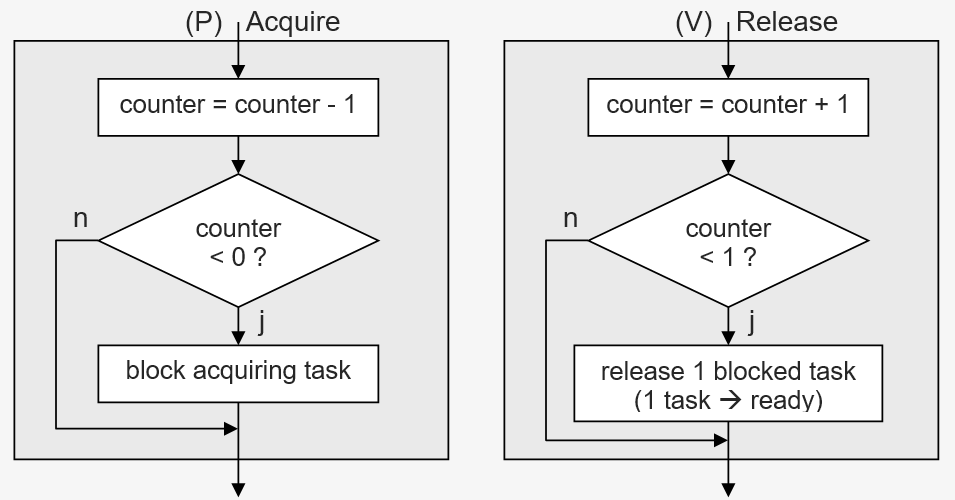
\includegraphics[width=12cm, height=5cm]{Images/image105.png}
    %\caption{}
    \label{fig:Fig 51}
    \end{figure}

It is of crucial importance that the operations "Passieren" and "Verlassen" (as originally introduced by Dijkstra) are realized atomically, i.e. they cannot be interrupted by any other operation. Only then, a consistent handling of the counter variable is ensured. Semaphore objects are managed by the RT-OS.\\

\textbf{Other names} for the \textbf{semaphore operations}:

P(sem) = Passieren(sem) = sem.P() = sem.decrement() = sem.wait() = take(sem)${}_{VXWorks}$

V(sem) = Verlassen(sem) = sem.V() = sem.increment()  = sem.signal() = give(sem)${}_{VXWorks}$\\


For \textbf{mutex-synchronization} a semaphore is used, with counter initialized with 1. Therefore, only one task can pass, gaining access to the protected resource: 

 	\begin{figure}[h]
    \centering
    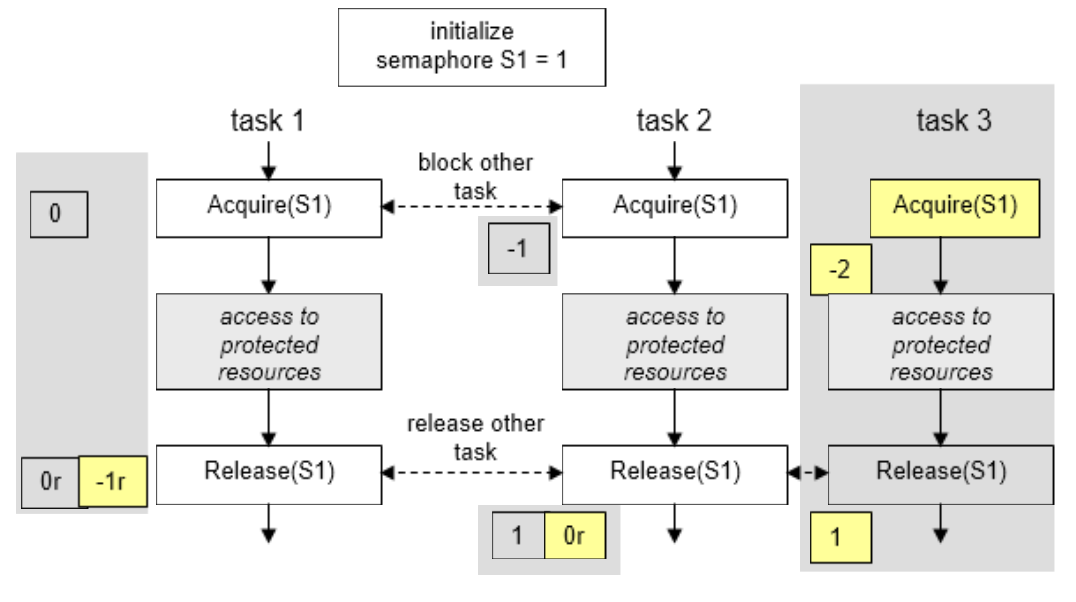
\includegraphics[width=14cm, height=7cm]{Images/image106.png}
    %\caption{}
    \label{fig:Fig 52}
    \end{figure}


\textbf{Example: Semaphore as Mutex in FreeRTOS}

\begin{lstlisting}[style=mystyle, language=c]
xSemaphore semAD;									// a global Semaphore
int table[16];										// a table of 16 temperatures

void vAppTask(void * pvParameters)
{
	semAD = vSemaphoreCreateBinary();		// Create a Semaphore, initially 1 

	while(1) {
		...
		xSemaphoreTake(semAD,portMAX_DELAY);		// <---- sync aquire mutex
		
		// read temperatures exclusicely ...
		Read_Temperatures(table);

		xSemaphoreGive(semAD,portMAX_DELAY);		// <---- sync release the mutex
 	}
}

void vPrintTask(void * pvParameters)
{
	while(1) {
		...
		xSemaphoreTake(semAD,portMAX_DELAY);	// <---- sync aquire mutex
		
		// print the table of temperatures exclusicely ...
		Print_Temperatures(table);

		xSemaphoreGive(semAD,portMAX_DELAY);	// <---- sync realease the mutex !
 	}
}
\end{lstlisting}

A \textbf{cooperation synchronization} can be realized by means of two semaphores. Example: sequential order of a task cooperation T2T1T2 with 2 semaphores:

 	\begin{figure}[h]
    \centering
    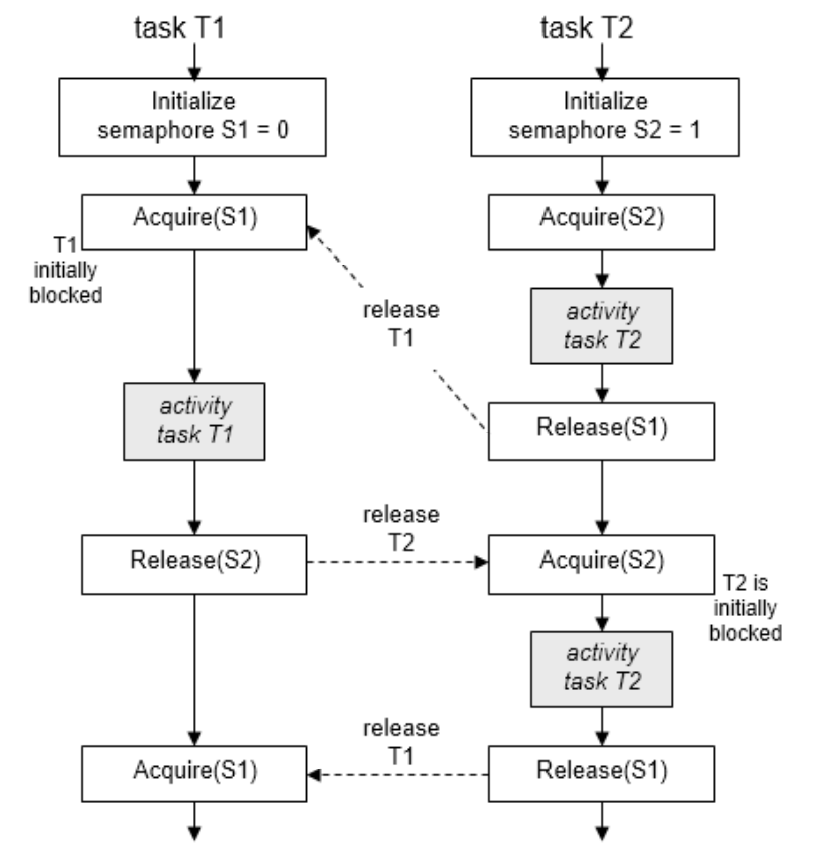
\includegraphics[width=11cm, height=10cm]{Images/image107.png}
    %\caption{}
    \label{fig:Fig 53}
    \end{figure}
\newpage
\os{\newpage}
\textbf{Example: Cooperation in FreeRTOS  }

\begin{lstlisting}[style=mystyle, language=c]
void init()
{
	s1 =	vSemaphoreCreateBinary();			// Create a binary Semaphore 
	s2 =	vSemaphoreCreateBinary();			// Create a binary Semaphore 
	initSemaphore(s1,0);  	
	initSemaphore(s2,1);
}

void vTask1(void * pvParameters)
{
	while(1) {
		xSemaphoreTake(s1,portMAX_DELAY);	// <---- sync take blocks task !
		t1_activity();						// main T1 activity
		xSemaphoreGive(s2,portMAX_DELAY);	// <---- sync 
 	}
}

void vTask2(void * pvParameters)
{
	while(1) {
		xSemaphoreTake(s2,portMAX_DELAY);	// <---- sync take blocks task !
		t2_activity();						// main T1 activity
		xSemaphoreGive(s1,portMAX_DELAY);	// <---- sync 
 	}
}
\end{lstlisting}

\subsection{Deadlocks}

Synchronization of tasks can lead to a deadlock (\textbf{\textit{block}}, \textbf{\textit{deadly embrace}}), a situation, where the continuation of one or more tasks is blocked permanently. A simple example of a deadlock is an intersection with right-before-left right-of-way rule and four simultaneously arriving vehicles. After the priority rule any vehicle must wait for being right to another one, none of the Vehicles can drive. Only a break of the rule can release the deadlock.In task management, there are two types of deadlocks: deadlocks and live locks.\\

In a deadlock tasks waiting on the release of resources for which they block each other. This leads to a standstill of the waiting tasks. The previous example with the traffic intersection describes such a deadlock.\\

Deadlocks typically occur when multiple resources are to be protected at the same time over cross:

\begin{figure}[h]
\centering
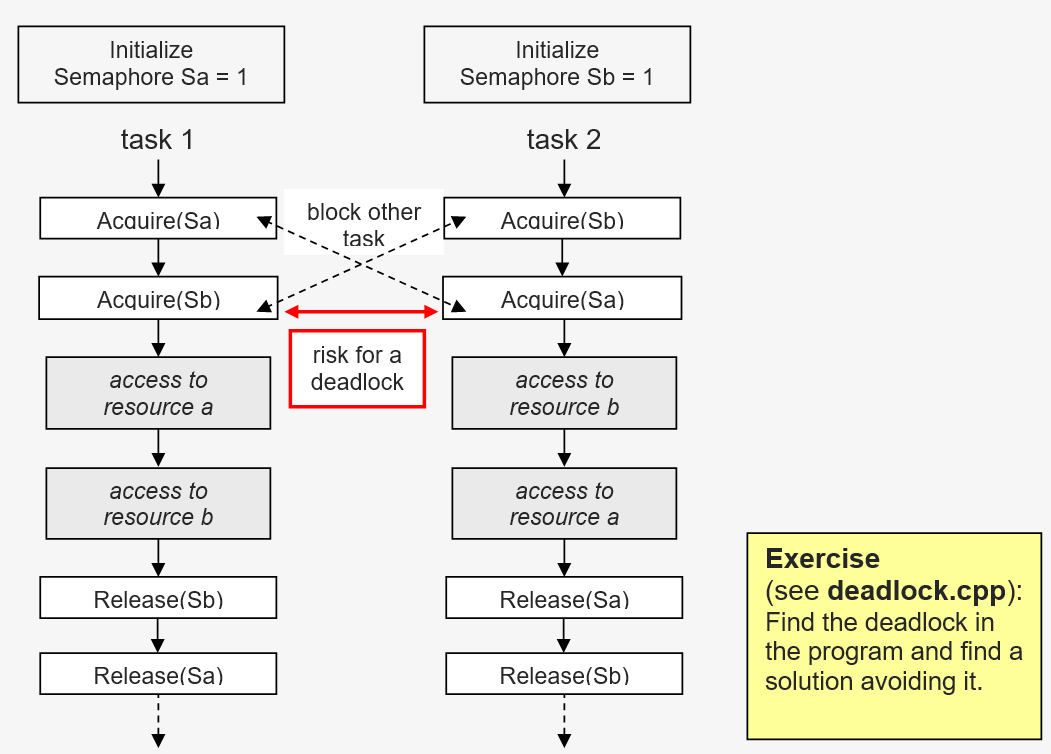
\includegraphics[width=11cm, height=10cm]{Images/image108.png}
%\caption{}
\label{fig:Fig 54}
\end{figure}

\nsl{In the above program there is a risk for a deadlock, since whenever both tasks are executed nearly parallel in time, both semaphores Sa and Sb are acquired, but never released. Deadlocks are usually realized unintended, i.e. as \textbf{\textit{software bugs}} !\\}

A simple rule to avoid deadlocks:

\begin{tcolorbox}[colback=blue!5!white,colframe=blue!75!black]
	If several resources are to be protected at the same time, all accessing tasks must acquire / release semaphores in the same order to avoid deadlocks.
\end{tcolorbox}

\nsl{Another, although less elegant, method is to remove deadlocks already occurred, by a defined waiting period for any task in blocked state, a so-called \textbf{\textit{time-out}}. If, after the time-out, a task is still in blocked state, that task is reset and all depending resources it occupied are released. This technique is implemented in some RTOSes, see also $\rightarrow$ Software Watchdog concept.}

\subsection{Livelocks}

Livelocks (starvation) designate a condition in which a task is constantly inhibited from running by the conspiracy of other tasks. For example, when using a fixed lower-priority task never can get the processor due to the constant activity of higher-priority tasks.\\

\textbf{Example} FPP, task 1\textbf{: high priority}, task 2:\textbf{ low priority}, task 3:\textbf{ medium priority}

\begin{figure}[h]
\centering
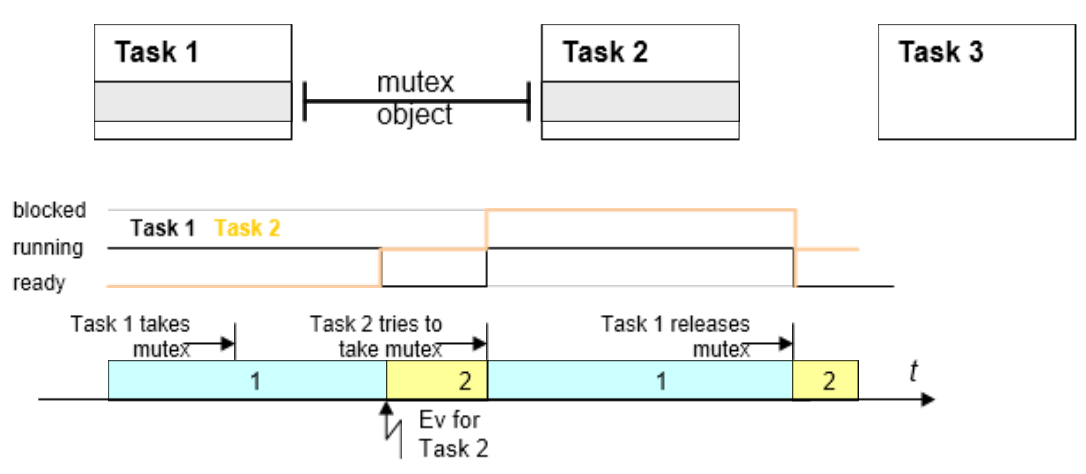
\includegraphics[width=12cm, height=6cm]{Images/image109.png}
%\caption{}
\label{fig:Fig 55}
\end{figure}

However, this can also happen in high-priority tasks, provided that a \textbf{\textit{priority inversion}} occurs: the high-priority task 1 is livelocked by the lower priority tasks 2 and 3:

\begin{figure}[h]
\centering
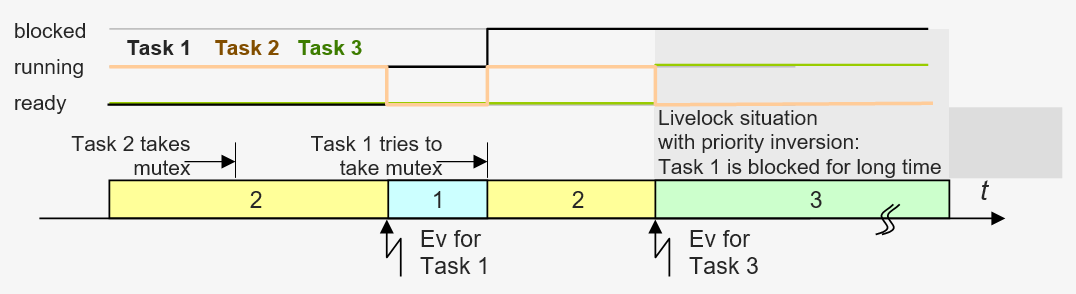
\includegraphics[width=12cm, height=4cm]{Images/image110.png}
%\caption{}
\label{fig:Fig 56}
\end{figure}

\newpage
The problem of livelock by priority inversion can be solved by the technique of \textbf{priority} \textbf{inheritance} [W\"{o}rnB]   in the example above: task 2 inherits the high priority of task 1 (both wait for the same mutex), such that task 2 running in the critical section cannot be interrupted by a medium priority task 3. \\

\nsl{A priority inversion condition occurs when a high-priority task must wait for synchronization objects of a lower-priority task (with \textbf{fixed priority scheduling}). This was the problem of the 1997 Mars mission "Sojourner" (running VxWorks), which was finally rescued by a watchdog [W\"{o}rnB].}

\subsection{Task Communication}

Synchronization and communication tasks are very closely related. \textbf{Synchronization} can be thought of as\textbf{ communication without information}. On the other hand, communication can be used for synchronization.\\

\nsl{An example could be waiting for an order. With the order, information is transmitted, and by the time the order is sent, synchronization is possible (the job can start actually).\\}

There are two basic variants of the task communication:

\begin{enumerate}
	\item  \textbf{Shared memory: } \\
	The data exchange is via a shared memory.\\
	The synchronization at what time read or write access occurred is done by a semaphore.
	\item  \textbf{Messages (Events): }The data exchange and synchronization is done via sending messages.
\end{enumerate}

In general, the communication via shared memory is faster than communication via messages. Therefore, this variant is preferred used in real-time operating systems. In spatially \textbf{\textit{distributed systems}}, this is not possible because there is no physically shared memory. Here communication must take place via messages ($\rightarrow$ message queues).
\newpage
\subsection{Events}

With a mutex synchronization the access of competing tasks to a jointly used resource was enabled. In contrast, for cooperating tasks time (and order) of execution has to be synchronized. This can be done by semaphores, but also with a simpler concept, an \textbf{\textit{event}}.\\

A task can wait on an \textbf{\textit{event}} (event wait), which is set by another task. Once set, the waiting tasks gets released from its blocking state.\\

\textbf{Example}: \\
Each of 3 tasks (task A, task B, task C) acquires a measurement value, which shall be processed by a 4${}^{th}$ task W. If A, B or C has acquired a measurement value, this is written to a data memory ("datenspeicher"), which can store exactly one value. Task W retrieves its input from that data memory.

 	\begin{figure}[h]
    \centering
    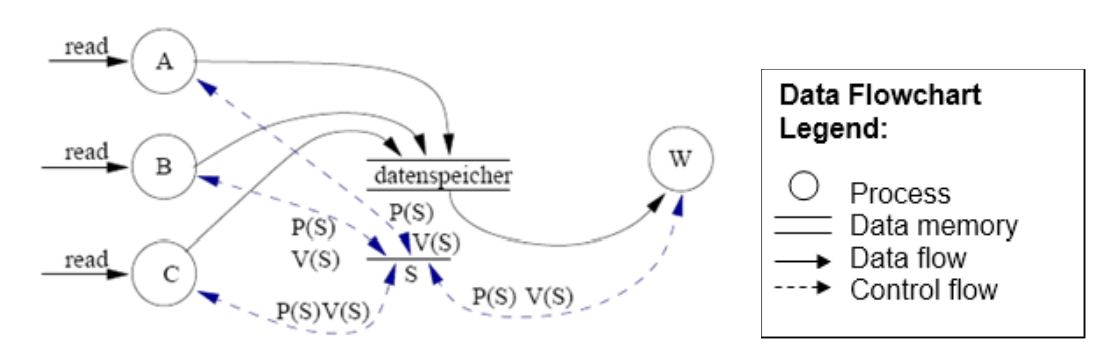
\includegraphics[width=13cm, height=4cm]{Images/image111.png}
    \caption{Data flow of an acquisition of measurement values: synchronization without events}
    \label{fig:Fig 57}
    \end{figure}
\os{\newpage}

Since the data memory  is existing only once, it is a shared resource, and access to it is a critical section, which can be protected by a semaphore S\\

\begin{lstlisting}[style=mystyle, language=c]
// Task A,B und C
	...
	while( TRUE ) {
  	read(kanal_A, buffer, sizeof(buffer));
  	P(S); // enter critical section
  	write( datenspeicher, buffer, sizeof(buffer));
 	 V(S); // leave critical section
}
...
\end{lstlisting}

\begin{lstlisting}[style=mystyle, language=c]
// Task W
while( TRUE ) {
  	P(S); // enter critical section
 	 read(datenspeicher, buffer, sizeof(buffer));
  	V(S); // leave critical section
 	 WorkOnData( buffer );
}
\end{lstlisting}

\textbf{Problems} with synchronization without events:

\hspace{1cm} \textbf{Data memory} can be overwritten, without being read before by W
 
\hspace{1cm} W can read the \textbf{data memory} repeatedly.\\

Therefore, it is not sufficient to protect the shared resources by using a semaphore, yet another synchronization means is necessary: an \textbf{\textit{event}}.

\begin{tcolorbox}[colback=blue!5!white,colframe=blue!75!black]
 \textbf{Definition: }\\ An \textbf{event} is a synchronization object, which allows computing processes to give free the processor (by going to the \textbf{block}-state), up to a certain condition is met.
\end{tcolorbox}

\textbf{Basic operations} of the \textbf{event} are:\\

\hspace{1cm}  Wait for an event, and

\hspace{1cm}  Send an event.\\

An \textbf{event} can\textbf{ get "lost"}, if an event is sent when no process waits on it  !\\
Since events are not stored -unlike semaphores-, events are used often in combination with a semaphore.
\os{\newpage}

\begin{figure}[h]
\centering
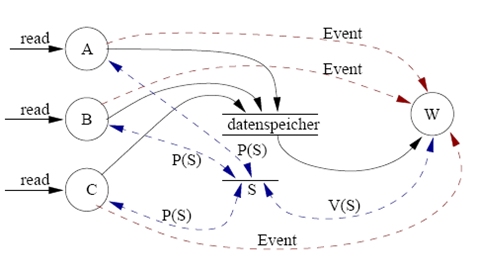
\includegraphics[width=10cm, height=4.5cm]{Images/image18.png}
%\caption{}
\label{fig:Fig 58}
\end{figure}

Data flow of an acquisition of measurement values: synchronization with events

In order to grant access to the data for the tasks A, B or C only, after task W has emptied the data memory, the operation "enter critical section" and "leave critical section" is distributed to different tasks, similar to cooperation synchronization with semaphores.\\

Each of the tasks A, B and C enters the critical section (by calling the "P(S)"-operation), but never "leaves the critical section" by itself, this release is now done by task W (by calling the "V(S)"-operation). Task W must now be synchronized, so that it fetches the data from memory only, if these are available. Thus, Task A, B or C send an event on which task W is waiting:\\

\begin{lstlisting}[style=mystyle, language=c]
// Task A,B und C
...
read(kanal_A, buffer, sizeof(buffer) );
P(S); // enter critical section
write( datenspeicher, buffer, sizeof(buffer) );
SendEvent( Task_W );
...
\end{lstlisting}

\begin{lstlisting}[style=mystyle, language=c]
// Task W
while (1) {
  WaitForEvent( Task_W );
  read( datenspeicher, buffer, sizeof(buffer) );
  V(S); // leave critical section after read
  WorkOnData( buffer );
}
\end{lstlisting}

The critical section is thus defined from the time which an acquiring task A,B, or C writes a value into the data memory, until task W has read the value out of the memory.\\
\os{\newpage}

\textbf{Problem}: Events can get lost, if sent when no task is waiting

 	\begin{figure}[h]
    \centering
    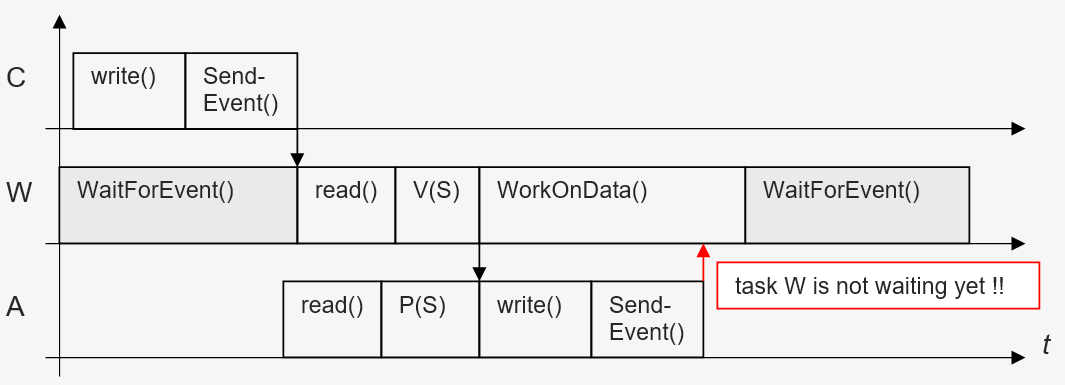
\includegraphics[width=14cm, height=4.5cm]{Images/image112.png}
    %\caption{}
    \label{fig:Fig 59}
    \end{figure}

\begin{itemize}
	\item task C causes task W to get running, starting with read()
	\item During read() in task W, task A has read new data
	\item task A is blocked by P(S), before W could release the semaphore
	\item task W releases V(S)
	\item task A continues with write() and SendEvent()
	\item the event gets lost, cause task W is busy WorkingOnData(), not waiting:  \textbf{\textit{critical race condition !!}}
	\item data loss A.
\end{itemize}
\nsl{\newpage}

\textbf{Solution}: Move he WorkOnData() call into the critical section:

\begin{lstlisting}[style=mystyle, language=c]
// Task W
while (1) {
  WaitForEvent( Task_W );
  read( datenspeicher, buffer, sizeof(buffer) );
  WorkOnData( buffer );
  V(S); // leave critical section after work
}
\end{lstlisting}

Now, with this solution, the conflict is solved, since immediately after the critical section is left, task W can wait for events there is no more critical race condition:

 	\begin{figure}[h]
    \centering
    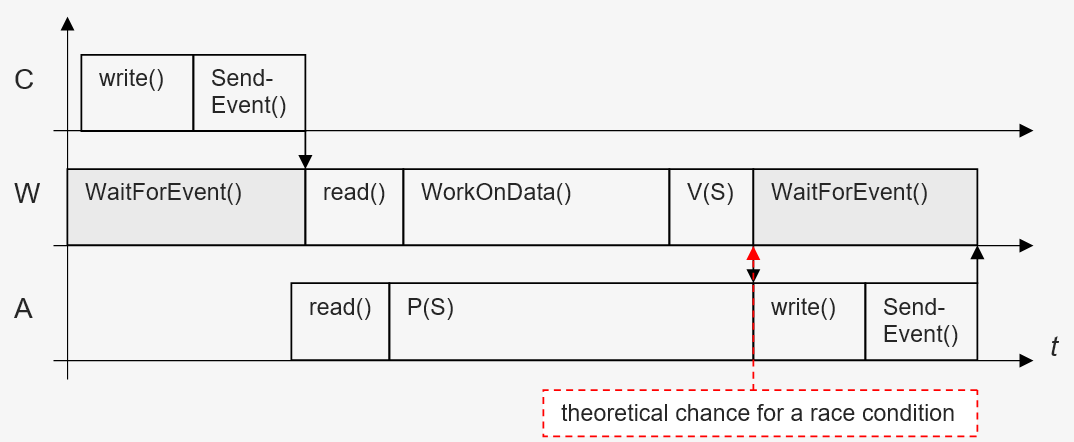
\includegraphics[width=14cm, height=4cm]{Images/image113.png}
    %\caption{}
    \label{fig:Fig 60}
    \end{figure}

Since there is a theoretical (although very small) chance, \textbf{Posix} defines an atomar, non-interruptable operation combining the semaphore release and waiting on an event:

 	\begin{figure}[h]
    \centering
    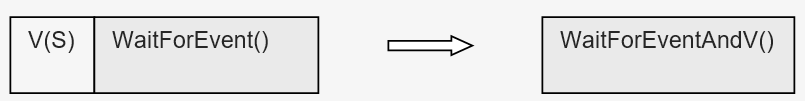
\includegraphics[width=10cm, height=1cm]{Images/image114.png}
    %\caption{}
    \label{fig:Fig 61}
    \end{figure}
    
\begin{lstlisting}[style=mystyle, language=c]
// Task W
P(S); // since WaitForEventAndV releases a semaphore
      // this most be locked (acquired) first
while(1) {
  read( datenspeicher, buffer, sizeof(buffer) );
  WorkOnData( buffer );
  // V(S); leave critical section after work, done above
  WaitForEventAndV(S); // Release semaphore and wait
}
\end{lstlisting}

\begin{lstlisting}[style=mystyle, language=c]
// Task A,B und C
...
read(kanal_A, buffer, sizeof(buffer) );
P(S); // enter critical section
write( datenspeicher, buffer, sizeof(buffer) );
SendEvent( Task_W );
...
\end{lstlisting}
\nsl{\newpage}

\nsl{\textbf{Posix Functions:}\\

By these functions a critical section is entered, and left

P(S):  int \textbf{pthread\_mutex\_lock }( pthread\_mutex\_t * \textit{mutex });

V(S):  int \textbf{pthread\_mutex\_unlock}( pthread\_mutex\_t * \textit{mutex });\\


WaitForEventAndV(S):

int \textbf{pthread\_cond\_wait}( pthread\_cond\_t * \textit{cond }, pthread\_mutex\_t * \textit{mutex });

\textbf{Alternative Solution: increase Memory, use }Message Queues \textbf{as a standard solution !}}

\subsection{Signals}

Signal are very similar to events. Signals can be processed asynchronously to the program (call of a signal-handler routine), with events the processing is synchronous (\textbf{wait\_for\_event}() - functions as part of the program).

\begin{itemize}
\item Signals are often used in UNIX programs. 
\item Signals they can be seen as software interrupts at the application level.
\end{itemize}

\subsection{Messages Queues, Mailboxes}

\textbf{Message queues} provide an asynchronous communication protocol, which means that the sender and receiver of the message must not interact simultaneously. Messages will be placed on a queue, where they are stored until the recipient retrieves one or more by a FIFO mechanism. The maximum amount of data a single message is usually limited.\\

A message queue without a restriction for the number of messages is called \textbf{mailbox}.

 	\begin{figure}[h]
    \centering
    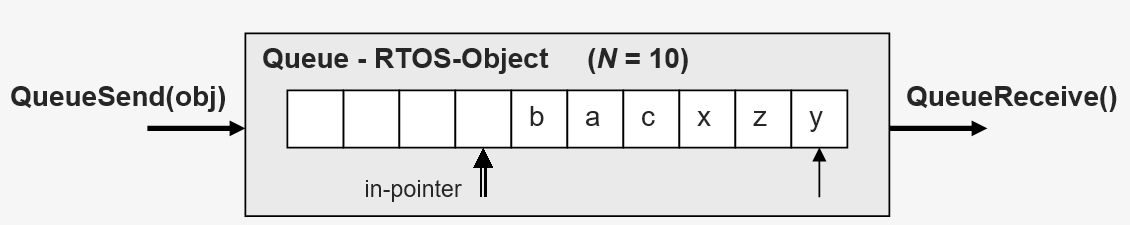
\includegraphics[width=14cm, height=3cm]{Images/image115.png}
    %\caption{}
    \label{fig:Fig 62}
    \end{figure}
\nsl{\newpage}    
\textbf{Example}: FreeRTOS - Queue (www.freertos.org)
\os{\newpage}

\begin{lstlisting}[style=mystyle, language=c]
#include <FreeRTOS/queue.h>
...
struct AMessage
{
	portCHAR ucMessageID;
	portCHAR ucData[ 20 ];
}

xQueueHandle xQueue1;

void vATask(void *pvParameters)
{
	// Create a queue capable of containing 10 pointers to AMessage structures.
	// These should be passed by pointer as they contain a lot of data.

	xQueue1 = xQueueCreate( 10, sizeof( struct AMessage * ) );
}

...

// -------------------------  send from any task ----------------------------}
{
 	// Send a pointer to a struct AMessage object.  Don't block if the
  	// queue is already full.
 	struct AMessage *pxMessage;

 	pxMessage = \& xMessage;
	xQueueSend( xQueue1, (void *) \&pxMessage, (portTickType) 0 );
}
...

// ------------------------- receive with any task --------------------------}

{  
	// Receive a message on the created queue.  Block for 10 ticks if a
	// message is not immediately available.
	struct AMessage *pxMessage;
	if( xQueueReceive(xQueue1, \&(pxRxedMessage), (portTickType ) 10 ))
	// pcRxedMessage now points to the struct AMessage variable posted

}
\end{lstlisting}

The \textbf{QueueReceive()} command places the calling task into the blocked (waiting) state if the message queue is empty. If not, it returns the object to which the read (out) pointer points to, and the read (out) pointer set to the next message object.\\

The \textbf{QueueSend()} command places the calling task into the blocked (waiting) state only, if the message queue is full. If not, the object is being stored at the position the write (in) pointer references, and the pointer is set to the next free space in which the next transmitted (posted) message object is stored.\\

In many RTOS, a maximum blocking time can be specified (as with FreeRTOS). Lab-experiment "Message Queue with ARM LPC4357 $\mu$C (FreeRTOS)"

\subsection{Socket Interface}

The most important interface for inter-process communication on different computers connected via Ethernet, is the socket interface.\\ 

By using sockets, data can be exchanged between processes, which are located on different hosts (distributed system).\\ 

The socket interface provides access to TCP/IP (connection-oriented) and UDP/IP (connectionless) protocols for communications.\\

Once a socket connection between two processes has been established, the data can be exchanged with some basic system functions (open, read, write, close ...), the so called Sockets Service Primitives.

 	\begin{figure}[h]
    \centering
    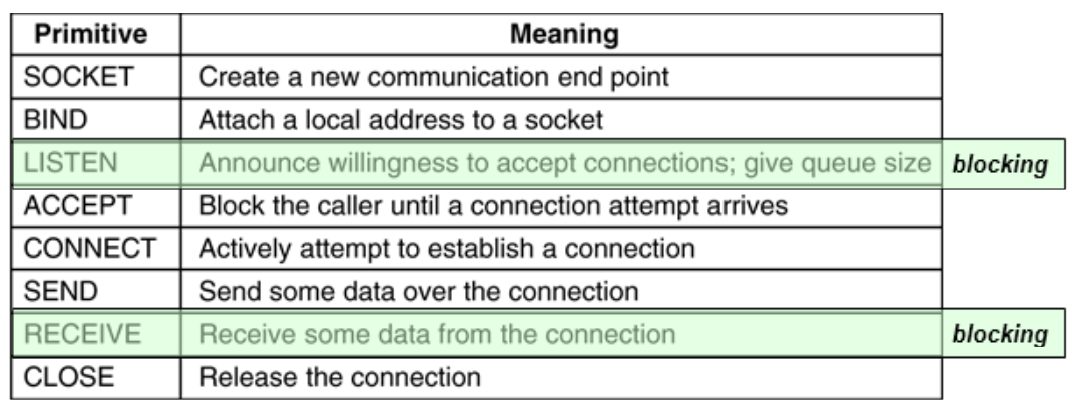
\includegraphics[width=12cm, height=5cm]{Images/image195.png}
    %\caption{}
    \label{fig:Fig 64}
    \end{figure}
    
RTP ProgC RepetitionWorkspace: "socket client, socket server"\\

{\rot \bf Python Sockets Programming}\\

The server connects to a client and echoes its message:

 	\begin{figure}[h]
    \centering
    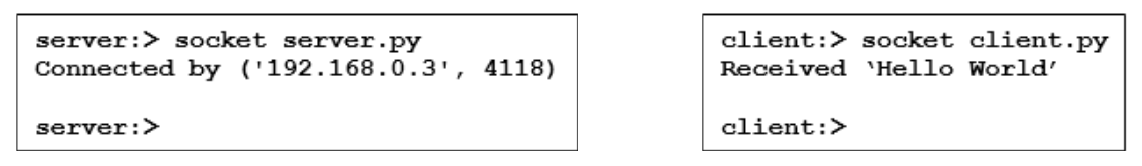
\includegraphics[width=14cm, height=2cm]{Images/image196.png}
    %\caption{}
    \label{fig:Fig 64}
    \end{figure}
\nsl{\newpage}

{\bf(A) Server script}\\

First, the server executes LISTEN (line 12), and it remains blocked until a client connects. Then a client task executes CONNECT to establish a connection with the server (line 9). It must specify an IP address (the server's) and port number (must me common to both).

 	\begin{figure}[h]
    \centering
    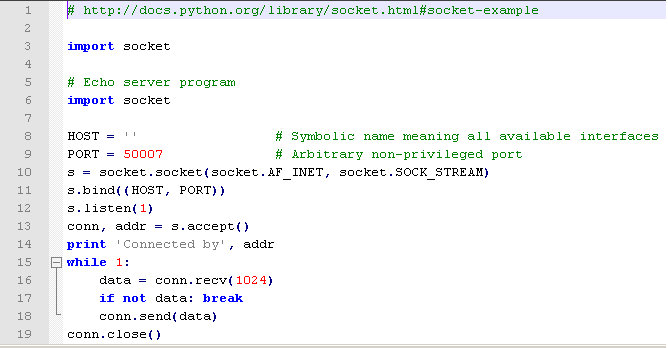
\includegraphics[width=14cm, height=6cm]{Images/image197.png}
    %\caption{}
    \label{fig:Fig 64}
    \end{figure}

{\bf(B) Client script}\\

 	\begin{figure}[h]
    \centering
    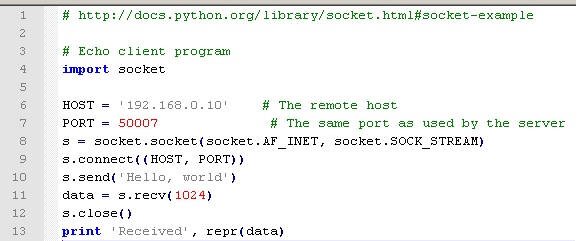
\includegraphics[width=14cm, height=6cm]{Images/image198.png}
    %\caption{}
    \label{fig:Fig 64}
    \end{figure}

The OS then sends an IP packet to the opposite computer (peer). The client process is blocked until the server responds. If a confirmation is received, the client and server have established a connection and the connect() - or listen() function are released from blocking, and data can be exchanged until the end of the connection (close()).
\nsl{\newpage}

\section{Memory Management}

The main task of memory management is essentially providing access to the memory resource consisting of a hierarchy of cache, main memory (RAM), peripheral memory or NVRAM (non-volatile RAM, such as EEPROM) by

\begin{itemize}
	\item  the allocation of memory to the tasks,
	\item  the coordination of accesses to shared memory areas,
	\item  the protection of the storage areas of individual tasks
	\item  the displacement of memory areas
\end{itemize}
\os{\newpage}

One can distinguish between different forms of memory allocation:

\begin{enumerate}
\item  \textbf{Static memory allocation: \\}The allocation of memory is made to a task before it is put into the \textbf{\textit{ready}} state. The memory allocation does not change at runtime.

\item  \textbf{Dynamic memory allocation: }\\The allocation of memory to a task is done at runtime and may change at any time.

\item  \textbf{Non-displacing memory allocation: }\\Allocated memory must not be withdrawn from a task at runtime.

\item  \textbf{Displacing memory allocation: }\\Allocated memory may be removed from a task at runtime, the memory is paged to peripheral memory (e.g. a swap-file).
\end{enumerate}

\nsl{\textbf{Embedded systems} mainly use \textbf{static memory allocation}, since the dynamic allocation of memory is hardly predictable (and thus real-time compliant).Execution times of \textbf{malloc(), free(), new(), delete()}, .. can't be guaranteed to be smaller than a certain limit  availability.\\}
\os{\newpage}

The usage of an \textbf{MMU} (\textbf{M}emory \textbf{M}anagement \textbf{U}nit), which is quite common with many CPUs (x86, ARM Cortex A Series, ..), allows processors to deal with a virtual address space. Thus, memory access from the process is strictly separated from the OS and from other processes (= safety). However, with translation of the virtual addresses into physikalical addresses long delays can occur, which cannot be determined in advance! This is a contradiction to the required determinism with hard real-time requirements ! Thus, microcontrollers for applications having hard real-time requirements often do \textbf{\underbar{NOT}}\underbar{ have an MMU} and use \underbar{direct physical addressing} instead (AVR, ARM Cortex M Series, ..) 

 	\begin{figure}[h]
    \centering
    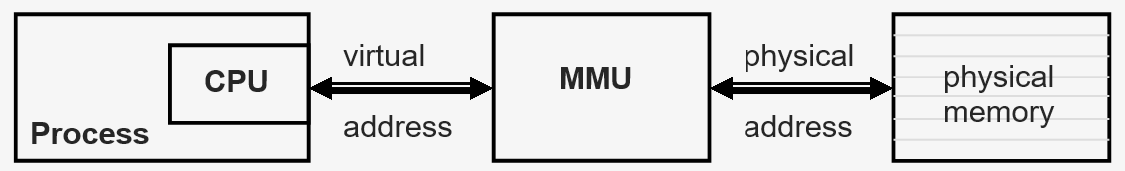
\includegraphics[width=12cm, height=2.5cm]{Images/image119.png}
    %\caption{}
    \label{fig:Fig 67}
    \end{figure}
    
\section{Input/Output Management (I/O)}

Along with task and memory management the\textbf{ }I/O management is the 3${}^{rd}$  important component of a real-time operating system, especially with embedded systems, where I/O tasks for sensors and actors have hard real-time requirements.\\

In addition to that, synchronous an asynchronous serial interfaces, and networking subsystems require high performance I/O-management.\\

{\rot\bf I/O Basics}\\

The tasks of the I/O-management can be divided into two groups:

\begin{itemize}
\item  Assigning and sharing of devices for the tasks
\item  Use of assigned and shared devices by the tasks
\end{itemize}

The connected devices differ greatly in speed and data format. The OS has therefore the task, to abstract from implementation details and provide a \textbf{simple, uniform and transparent interface}. \\

This can be achieved by a multi-layer architecture of the I/O management:

 	\begin{figure}[h]
    \centering
    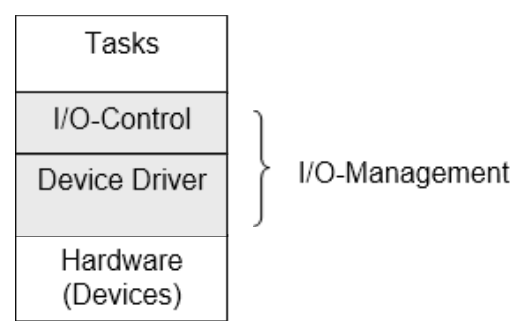
\includegraphics[width=6cm, height=4cm]{Images/image189.png}
    %\caption{}
    \label{fig:Fig 68}
    \end{figure}
    
The main 2 layers of I/O-management:

\begin{enumerate}
\item  \textbf{I/O-Control: }\nsl{\\This layer is above the layer of the device driver and interfaces with the tasks.It is hardware independent, i.e. implementation and operation is no longer depending on the type of connected devices. It takes care for data transport, data format, data buffering, and messaging. If a certain device needs to be exchanged, its device driver needs to be exchanged too, but not the I/O control.The I/O control abstracts from the specific devices and provides a \textbf{simple, uniform and transparent interface} to the \textbf{tasks}.}

\item   \textbf{Device Driver:}\nsl{\\The device driver is a layer next to the hardware, i.e. its realization depends on the connected devices. It takes into account all device-specific properties, including direct communication with the devices. It produces all necessary control signals, evaluates the status signals andhandles the device's interrupts. The device driver monitors all transfers, and possibly do some error handling, e.g. evaluate parity bits and initiate the repetition of a failed transmission.}
\end{enumerate}

\textbf{Example}: I/O-management of a hard disk drive:\\

\nsl{Each drive has a unique device driver, that takes into account their specific characteristics such as speed, number of heads, cylinders and sectors. At the level of I/O-control, each disk is treated equally, for the task addressing of data is done by a block number, abstracted from the device-specific parameters: \\

\textbf{FILE *fp =  fopen("c:{\textbackslash}test.bin"); fseek(fp, {\dots}), fwrite(fp, {\dots}), fclose(fp);}\\}

Typical interface functions provided by the I/O control layer

\begin{table}[h!]
\setlength{\tabcolsep}{10pt} % Default value: 6pt
\renewcommand{\arraystretch}{1.5} % Default value: 1
\centering
 \begin{tabular}{|c|c|c|c|} \hline
 \textbf{Function} & \textbf{Description} \\ [0.1ex] 
Create & Creates a virtual instance of an I/O device \\ \hline 
Destroy & Deletes a virtual instance of an I/O device \\ \hline 
Open & Prepares an I/O device for use \\ \hline 
Close & Communicates to the device that its services are no longer required, which \\ & typically initiates  device-specific cleanup operations \\ \hline 
Read & Reads data from an I/O device \\ \hline 
Write & Writes data into an I/O device \\ \hline 
Ioctl & Issues control commands to the I/O device (I/O control) \\ \hline 
 \end{tabular}
 %\caption{\textbf{}}
 %\label{Intrinsic}
\end{table}

The main functions of the I/O control layer are:

\begin{enumerate}
\item  \textbf{Symbolic Names: }devices addressing by symbolic addresses, or names.
\item  \textbf{Handling of I/O-Requests: }queuing, buffering I/O-requests  queues.
\os{\newpage}
\item  \textbf{Assignment of Devices: }assignment of the device (shared resource) to tasks dynamically or 	statically,using priorities for competing requests. 
\item  \textbf{Synchronization: }I/O-requests affect a tasks state, (e.g. waiting  \textbf{\textit{blocked}} state), interface between I/O-control to task-management.
\item  \textbf{Device Protection: } prevent unauthorized access by unauthorized tasks - protection against deadlocks and livelocks due to competing access- resets after programmable timeouts (protect against software failure).
\item  \textbf{Communication with the device drivers: }forwarded executable device requests to the device driver, handle feedback, e.g., status or error codes 
\item  \textbf{Buffering: }synchronization of different speeds of task-management and I/O-devices by temporary storage in buffer memory, handle buffter state events to the task/device
\item  \textbf{Unique Data Format: }abstract from the device's physical data format, e.g. \textbf{endianness}.
\end{enumerate}

The boundary between I/O control and device drivers is floating and system dependent. For efficiency reasons with some RTOSes, functionality is moved into the device driver, which increases the effort for adapting new devices.\\

{\rot\bf Endianness}\\

The storage of the hexadecimal number 0x0A0B0C0D = 168496141 results in a different byte order in memory, dependent of the microcontroller or peripheral hardware:

 	\begin{figure}[h]
    \centering
    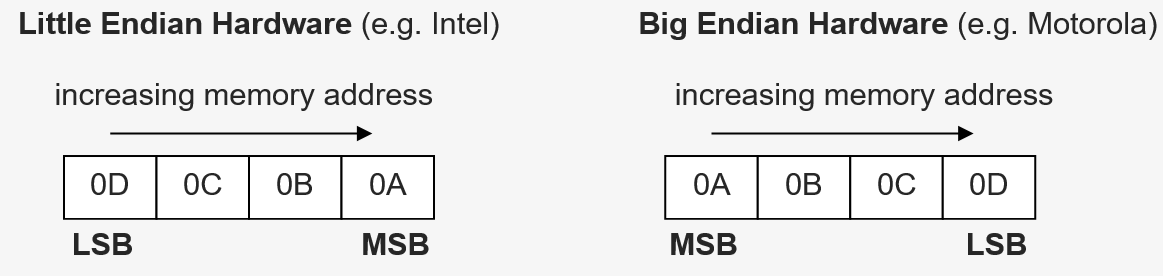
\includegraphics[width=13cm, height=2.5cm]{Images/image120.png}
    %\caption{}
    \label{fig:Fig 69}
    \end{figure}

\begin{enumerate}
\item  With \textbf{little-endian} hardware the least significant byte (\textbf{LSB}) is stored with the \textbf{lowest} \textbf{memory} (byte) \textbf{address}, 

\item  With \textbf{big-endian} hardware the most significant byte (\textbf{MSB}) is stored with the \textbf{lowest} \textbf{memory} (byte) \textbf{address}
\end{enumerate}

\nsl{Most RTOS's provide functionality to abstract from \textbf{endianness} in the device driver. Example:

 	\begin{figure}[h]
    \centering
    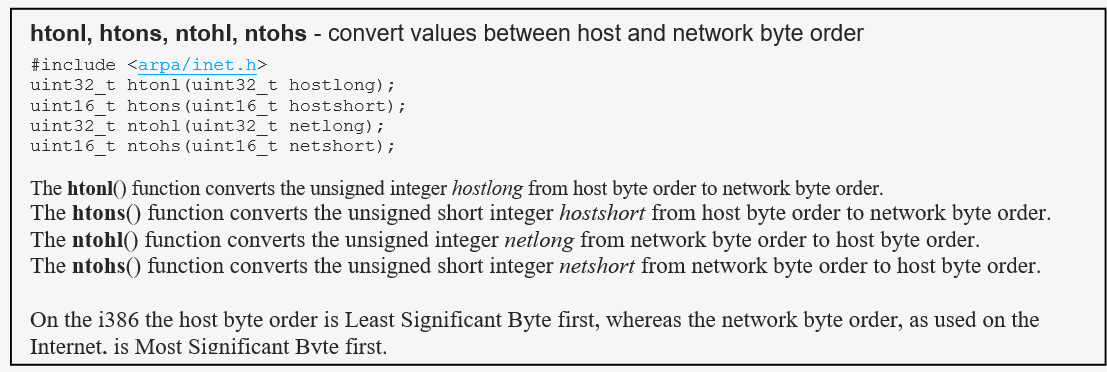
\includegraphics[width=14cm, height=6cm]{Images/image121.png}
    %\caption{}
    \label{fig:Fig 70}
    \end{figure}}

\subsection{I/O Synchronization}

The communication between peripheral devices and the processor is performed by interface devices. These \textbf{interface devices} also define the base for synchronization between the processor, and devices operating at different speeds using certain registers.

 	\begin{figure}[h]
    \centering
    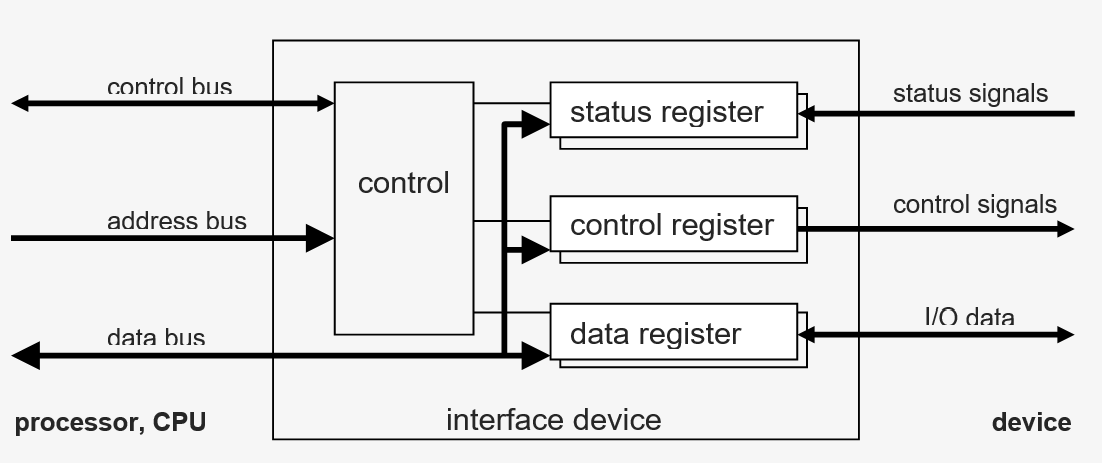
\includegraphics[width=10cm, height=4cm]{Images/image122.png}
    %\caption{}
    \label{fig:Fig 71}
    \end{figure}

The typical components of an interface device are:

\begin{enumerate}
	\item  \textbf{Data register} to read/write the data to be received/transmitted.
	\item  \textbf{Control register} for configuring the device (e.g. operating mode, speed of serial ports, UART).
	\item  \textbf{Status register} reflecting the devices current state (e.g. sent/received data bits, ADC).
\end{enumerate}

\nsl{A running task can synchronize  (for changing data) with the interface device either by

\begin{enumerate}
	\item  Polling
	\item  Interrupts
\end{enumerate}}

\subsection{Polling}

With the simplest synchronization method polling a task reads the status register continuously in a loop:
\nsl{\newpage}
 	\begin{figure}[h]
    \centering
    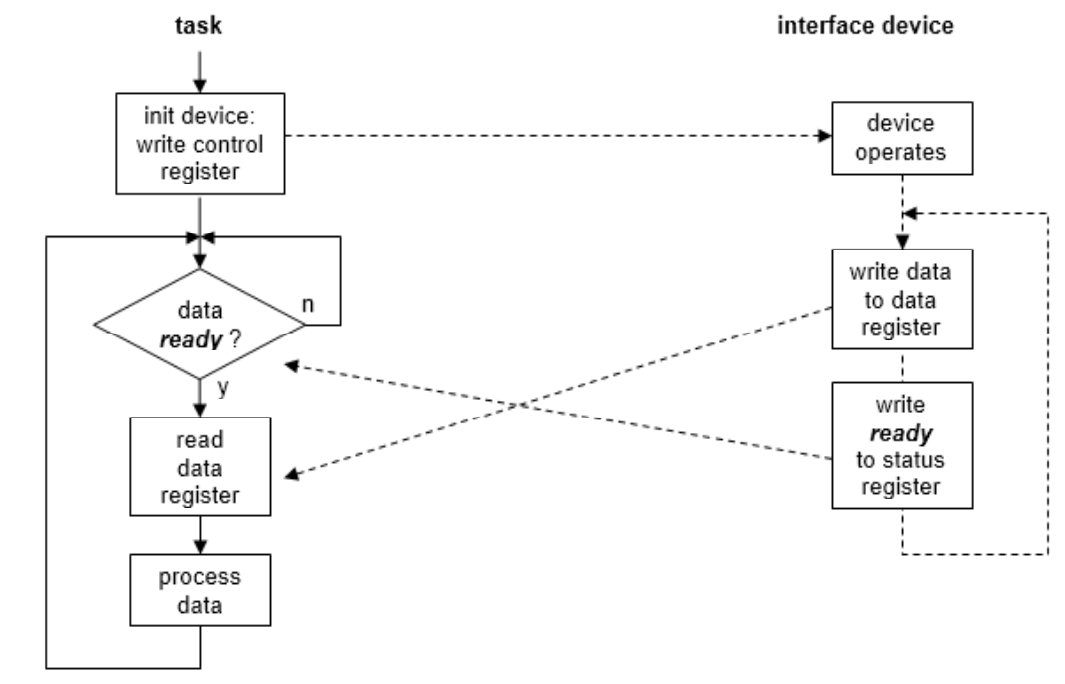
\includegraphics[width=14cm, height=10cm]{Images/image123.png}
    %\caption{}
    \label{fig:Fig 72}
    \end{figure}

After initialization (by setting the control register) the task is waiting in an active loop on a status flag which is a particular bit within the status register of the device indicating that  data is available in the data register. The task reads the data from the data register.\\

\textbf{Advantages}

\begin{itemize}
\item Simple synchronization type
\end{itemize}

\textbf{Disadvantages}

\begin{itemize}
\item Consumption of processor time for the active loop
\item Slow response times when multiple devices within a task are polled simultaneously.
\end{itemize}

\textbf{Conclusion}: Overall, polling is usually not favourable, due to inefficient CPU usage.\\
\newpage
\subsection{Busy Polling}

With busy polling, the properties of simple polling are improved with performing some activity (typically short) within the waiting loop:

 	\begin{figure}[h]
    \centering
    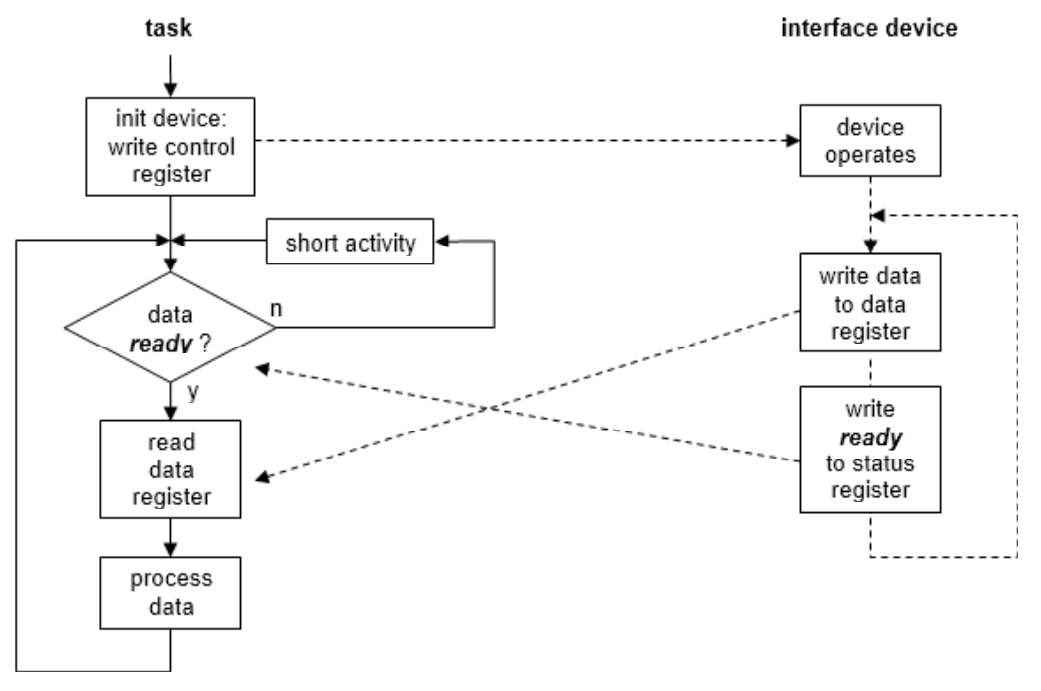
\includegraphics[width=14cm, height=9cm]{Images/image124.png}
    %\caption{}
    \label{fig:Fig 73}
    \end{figure}

A disadvantage is, however, the response time slows down. Longer activities must be split into smaller steps.\\

\textbf{Example (sampling system }(PWM-Control Experiment in Real-Time-Lab): 

\begin{itemize}
	\item  Start an AD converter process with known duration, 
	\item  Offset / Gain correction of previously read values,
	\item  Wait for the ADC to get ready,
	\item  Readout of the ADC data register.
\end{itemize}

 	\begin{figure}[h]
    \centering
    \includegraphics[width=6cm, height=4.5cm]{Images/image125.png}
    %\caption{}
    \label{fig:Fig 74}
    \end{figure}
\newpage
\subsection{Interrupts}

With synchronization by interrupts the interface executes an interrupt request with the processing CPU, which forces a currently running task to be interrupted in favor of a defined interrupt service routine \textbf{ISR}:

 	\begin{figure}[h]
    \centering
    \includegraphics[width=14cm, height=9cm]{Images/image126.png}
    %\caption{}
    \label{fig:Fig 75}
    \end{figure}

In the interrupt service routine (ISR), the data can be read from or written to the device.\\

\textbf{Advantage: }

\begin{itemize}
\item Processing time is consumed only, when data needs to be transferred
\end{itemize}

\textbf{Disadvantage: }
\begin{itemize}
\item Activating the ISR causes an overhead as the current processor state must be    saved for the old task to resume after return of the ISR    (equivalent to pre-emption with task-scheduling).
\item To reduce the effect of overhead, larger amounts of data are transmitted in blocks, usually in conjunction with direct memory access (DMA).
\item .The technique of synchronization with interrupts is very well suited for real-time applications and thus interrupts are widely used with micro-controllers with both synchronous and asynchronous real-time programming.
\end{itemize}

\os{\newpage}
\subsection{Interrupts and Task-Scheduling}

\nsl{Interrupt handling in real-time operating systems raises the question, how these interruptions integrate with the task scheduling. On current processor CPUs a hardware interrupt causes the automatic invocation of an interrupt service routine (ISR). \\}

The real-time operating system then has two options:

\begin{enumerate}
\item {\rot\bf Interruption of the Task-Oriented Processing: }

\begin{itemize}
	\item With an interrupt the currently running task is interrupted. The interrupt service routine (ISR) is executed immediately, after return the interrupted task continues.
\end{itemize}

\textbf{Advantage: } 

\begin{itemize}
	\item Very fast response to external events, because the interrupts are handled directly   by the CPU hardware.
\end{itemize} 

\textbf{Disadvantages: }

\begin{itemize}

\item The regular task-scheduling (eg EDF, FPP, TSS ...) is bypassed by direct handling   of the processor hardware.

\item The prozessor uses its own priority based preemption (FPP), might conflicting with real-time scheduling

 	\begin{figure}[h]
    \centering
    \includegraphics[width=14cm, height=5cm]{Images/image22.png}
    %\caption{}
    \label{fig:Fig 76}
    \end{figure}

\item Regardless of the scheduling strategy used by real-time scheduling events are treated with FPP scheduling, which can not guarantee 100\% processor utilization   (see section 2.2.7).

\item This kind of direct processing of interrupts with interruption of the task-oriented   processing is used for RTOS's with less performant microcontrollers,   better solution: integration of interrupts with task-scheduling.- The total available processor utilization for task-scheduled processing is reduced from originally 100 \% !
\end{itemize}
\os{\newpage}
\item {\rot\bf Integration of Interrupts with the Task-Oriented Processing: }\\

There is a separate task, integrated with task-scheduling, which is responsible for interrupt processing. Thus, whenever the processor gets a hardware interrupt, the ISR starts that separate task, responsible for interrupts.\\

\textbf{Advantage: }

\begin{itemize}
	\item Interrupt handling is fully integrated with task-scheduling,   there are no more two schedulers simultaneously, which might conflicting.
	\item An interrupt has the same scheduling policy as all other tasks.   (e.g. an interrupt can have lower priority than the actually running task, such that it   is not interrupted, with solution 1, this is not possible).
\end{itemize}  

\textbf{Disadvantage: } 

\begin{itemize}
	\item The reaction to events is slowed, because the interrupt handling is not activated   directly by hardware any more, but by the task-scheduler.
\end{itemize} 

 	\begin{figure}[h]
    \centering
    \includegraphics[width=14cm, height=5cm]{Images/image23.png}
    %\caption{}
    \label{fig:Fig 77}
    \end{figure}
\os{\newpage}
The integration of interrupts into the task-oriented processing is suitable for real-time operating systems using more powerful micro-controllers.
\end{enumerate}
\nsl{\newpage}

\section{Specialized RTOS}

\subsection{ Overview of some RTOS}

 	\begin{figure}[h]
    \centering
    \includegraphics[width=15cm, height=9cm]{Images/image127.png}
    %\caption{}
    \label{fig:Fig 78}
    \end{figure}

\subsection{ Classification of Real-Time Operating Systems}

For classifying RTOSes there can be made a separation into five basic types:

\begin{enumerate}
\item  \textbf{Minimal Real-Time Operating System (MinOS)} 

\begin{itemize}
	\item Simple RTOS for microcontroller with limited memory resources.
	\item RTOS is a library, to be linked with the application.
	\item Simple I/O-functions No memory management, physical addressing only (no protected mode).
	\item threads only (lightweight processes)
\end{itemize}

\item  \textbf{Controller System (CS)} 

\begin{itemize}
	\item Minimal real-time operating system 
	\begin{itemize}
	\item File system
	\item Better error handling.
	\end{itemize}
\end{itemize}
\os{\newpage}
\item  \textbf{Dedicated System (DS)}   
\begin{itemize}
	\item  Controller System
	\begin{itemize}
	\item Memory management.
	\item Protected mode
	\end{itemize}	     
\end{itemize}

\item  \textbf{Standard OS Extension (ExtOS)}
\begin{itemize}
	\item  Standard OS (Windows, Linux, ..)  
	\begin{itemize}
	\item Some RTOS features
	\end{itemize}
\end{itemize} 

\item  \textbf{Universal Real-Time OS (RTOS)} 
\begin{itemize}
\item  Fully featured RTOS.
	\begin{itemize}
	\item Features of standard OS.
	\end{itemize}
\end{itemize} 
\end{enumerate}

\subsection{Selection Criteria}

A first selection criterion is the classification described in 2.6, which is set by the scope and functionality of a real-time operating system (RTOS).Other criteria selecting an RTOS are:

\begin{enumerate}
\item  \textbf{Development and Target Environment}

\nsl{\begin{itemize}
	\item  Are there well-proven tools and libraries for both development and target ?
	\item Is the desired programming language supported (C, C++, ..) ?
	\item Smooth, reliable and fast communication process between the  target system and development system (re-flash cycle) ?
	\item What are the debug options and debugging tools on the target system  (E.g., source-level debugging)?
\end{itemize}}

\item  \textbf{Modularity and Core Size}

\nsl{\begin{itemize}
	\item  This criterion refers to the configuration and the memory requirements.
	\item Can the system be configured flexibly to the application ?
	\item Can it be restricted to the necessary components ? 
	\item What is the achievable size, application + libraries ?
\end{itemize}}

\item  \textbf{Adaptability}

\nsl{\begin{itemize}
	\item Is the RTOS adaptable for a particular microcontroller/peripherals ?
	\item How much effort is that adaption ?
	\item What field-bus systems or networks are supported ?
\end{itemize}}

\item  \textbf{General Features}

\nsl{\begin{itemize}
	\item What is the user interface of the operating system (GUI, cmd, None) ?
	\item Which libraries are part of the operating system ? (e.g. math, graphical)
	\item What other tools are offered, (e.g. for version management, data management)
\end{itemize}}

\item  \textbf{Performance}\\ \nsl{(usually a major criterion for selection). 
\begin{itemize}
	\item How large is the maximum number of tasks ?   (small automation app: 10 tasks, complex app: $\mathrm{>}$ 100 tasks)
	\item What task-scheduling methods are available ?
	\item What is the number of different priority levels ?
	\item What is the time for a context-switch ?
	\item What is the latency time with responding to interrupts ?
	\item For which class of real-time application the OS is designed ?  (e.g. can hard or firm real-time requirements be met ?)
\end{itemize}}
\end{enumerate}

\subsection{ VxWorks}

VxWorks, by Wind River Company [2004], is a general purpose real-time operating system. In in its basic form, it supports no virtual memory ( $\rightarrow$ advanced product VxVMI). VxWorks uses heavyweight processes as tasks. However, task-switch was optimized to enable fast task switching. The context VxWorks stores in a task-control block (TCB) includes:

\begin{enumerate}
\item  The program counter of the task,

\item  The contents of processor registers and floating-point,

\item  The stack of the dynamic variables,

\item  The associated I / O devices,

\item  The signal handler and

\item  Various debugging information
\end{enumerate}

The VxWorks state model for the tasks differs not much from the general model from section 2.1.3:

 	\begin{figure}[h]
    \centering
    \includegraphics[width=6cm, height=6cm]{Images/image128.png}
    %\caption{}
    \label{fig:Fig 79}
    \end{figure}

\begin{enumerate}
\item  \textbf{Running} the task is executed (run).

\item  \textbf{Ready} the task is ready to execute.

\item  \textbf{Blocked} (pending) the task is waiting for the release of a resource and is blocked.

\item  \textbf{Delay} (delayed) the task is stopped for a certain period of time.

\item  \textbf{Suspended} (suspend) the task was suspended. This is intended for debugging purposes only.
\end{enumerate}

By default, VxWorks uses FPP scheduling. Each task is assigned an initial priority. This priority can be adjusted during runtime ( function \textbf{taskPrioritySet}() ). VxWorks defines 256 priority levels, with 

\begin{enumerate}
\item  level \textbf{0} corresponding to the \textbf{highest}, and 

\item  level \textbf{255} to the \textbf{lowest priority}.
\end{enumerate}

The VxWorks task scheduler can be turned on and off explicitly by two functions (\textbf{taskLock() and taskUnlock()} ). The switch will prevent, that the current task is pre-empted by a higher priority task  realization of non-preemptive scheduling (FPN).\\

However, a task can still be interrupted by hardware interrupts. Deactivation of the task-scheduler is called \textbf{pre-emption locking}. It can be used for the protection of (short) critical sections. VxWorks also supports Time Slice Scheduling for tasks with equal priority.\\

\os{\newpage}
{\rot\bf Priority inversion}\\

With priority based scheduling the priority inversion problem can arise, which became popular with the mars pathfinder mission "Sojourner", 1997): \\

\textbf{Solution}: Priority Inheritance [1].\\

The priority-inheritance protocol assures that a\textbf{ task that holds a resource executes} at the \textbf{priority of the highest-priority task blocked} on that \textbf{resource}. In VxWorks the priority-inheritance protocol can be activated for a mutual-exclusion semaphore with the option \textbf{SEM\_INVERSION\_SAFE} enabled. \\

\os{\newpage}
For communication between tasks VxWorks provides the following mechanisms:

\begin{enumerate}
\item  Shared memory

\item  Signals

\item  Semaphore

\item  Message pipes

\item  Sockets to communicate with other computers via network

\item  Non-local procedure calls (Remote Procedure Calls) to other computers over the network.
\end{enumerate}

With VxWorks it is also possible to use libraries or program routines for several tasks simultaneously (shared code)  \textbf{reentrancy techniques}

\subsection{ FreeRTOS}

\textbf{FreeRTOS} is an Open-Source  real-time operating system for Embedded Systems. FreeRTOS was ported to a large number  of different micro-controllers with different performance.

 	\begin{figure}[h]
    \centering
    \includegraphics[width=3cm, height=2cm]{Images/image129.png}
    %\caption{}
    \label{fig:Fig 80}
    \end{figure}
    
\begin{itemize}
\item  Microcontrollers with ARM7-Architektur
\item  Microcontrollers of the ARM Cortex-M family (M0 {\dots} M4)
\item  Altera Nios II Softcore Processor
\item  Atmel AVR and Atmel AVR32
\item  Freescale Semiconductor HCS12-Familie and Coldfire V2
\item  Xilinx MicroBlaze and PowerPC PPC405
\item  Texas Instruments MSP430
\nsl{\item  Microchip Technology PIC18, PIC24, dsPIC, PIC32
\item  Renesas H8/S SuperH
\item  Fujitsu MB91460 32bit and MB96340 16bit
\item  NEC V850ES 32bit and 78K0R 16bit
\item  x86-Arcitecture}
\end{itemize}

\textbf{Features}\\

To ensure good maintainability, FreeRTOS is developed mostly in C, only a few functions are implemented in assembler. The scheduler can be configured for preemptive and cooperative operation. The OS (since version 4) supports two different task classes: "real" tasks and coroutines, the latter are recommended where little space is available.\\

\nsl{At www.FreeRTOS.org a very extensive documentation to \textbf{FreeRTOS}, tutorials and implementation examples realized on various microcontrollers.\\

\textbf{SafeRTOS} is a derivate of \textbf{FreeRTOS}, designed for safety-critical applications  by IEC 61508. \textbf{SafeRTOS} is cerified by \textbf{T\"{U}V S\"{u}d} up to SIL level 3.\\

\textbf{Example}: AD-DA Task of a Sampling Controller\\}

 	\begin{figure}[h]
    \centering
    \includegraphics[width=8cm, height=5cm]{Images/image131.png}
    %\caption{}
    \label{fig:Fig 81}
    \end{figure}
\newpage

\subsection{ FreeRTOS Task-Model}

 	\begin{figure}[h]
    \centering
    \includegraphics[width=9cm, height=6cm]{Images/image132.png}
    %\caption{}
    \label{fig:Fig 82}
    \end{figure}

\nsl{{\rot\bf FreeRTOS API-Funktionen (Selection)}\\

\begin{table}[h!]
\setlength{\tabcolsep}{10pt} % Default value: 6pt
\renewcommand{\arraystretch}{1.5} % Default value: 1
\centering
\begin{tabular}{|l|l|} \hline 
xTaskCreate() & Create a task \\ \hline 
vTaskStartScheduler() & Start Scheduler \\ \hline 
vTaskSuspend() &  \\ \hline 
vTaskResume() &  \\ \hline 
xTaskResumeFromISR() & Resume a suspended task by an ISR \\ \hline 
vTaskDelay() &                    \textit{blocking} \\ \hline 
vTaskDelayUntil() & \textbf{\textit{ suitable for exact real-time requirements !  }}\textit{blocking}\textbf{\textit{}} \\ \hline 
\textbf{\textit{}}vSemaphoreCreateBinary() & Create a binary Semaphore \\ \hline 
xSemaphoreCreateCounting() &  \\ \hline 
xSemaphoreCreateMutex()  & Create Mutex Objekt \\ \hline 
xSemaphoreGive() & give (release) a semaphore, V() operation \\ \hline 
xSemaphoreTake() & take (acquire) a semaphore, P()-operation    \textit{blocking} \\ \hline 
xQueueCreate() &  \\ \hline 
xQueueSend() &  \\ \hline 
xQueueReceive() &                    \textit{blocking} \\ \hline 
xTaskGetTickCount() & Ticks since the Scheduler was started ( WCET) \\ \hline 
\end{tabular}
%\caption{\textbf{}}
%\label{Intrinsic}
\end{table}

{\rot\bf FreeRTOS }\\
\begin{itemize}
\item Offers a "\textbf{Basic Priority Inheritence}" mechanism for mutex and semaphore objects for avoidance of \textbf{Livelocks}.
\item various student projects use FreeRTOS on ARM boards (or similar) at the Real-Time Programming department of the Hochschule Ravensvburg-Weingarten $\rightarrow$ template PingPong
\end{itemize}}

\os{\newpage}
{\rot\bf Lab Experiment PingPong}\\

Task diagram for 4 parallel running tasks (3 + 1 init):\\

 	\begin{figure}[h]
    \centering
    \includegraphics[width=13cm, height=9cm]{Images/image133.png}
    %\caption{}
    \label{fig:Fig 83}
    \end{figure}

\os{\newpage}
\begin{lstlisting}[style=mystyle, language=c]
// ----------------------------------------------------------------------------
/// \file		 PingPong.c
/// \brief		 RTP-Lab intro.
/// \author		 Wolfgang Schulter 
/// \license	 for educational purposes only, no warranty, see license.txt
/// \date		 14.01.2013 ws:  initial version
// ----------------------------------------------------------------------------

#include "PingPong.h"  				// PingPong module header

xSemaphoreHandle semPing;			// semaphore Ping
xSemaphoreHandle semPong;			// semaphore Pong

uint16_t count = 0;					// count variable incremented by ping

#define TICK_RATE_KHZ	(configTICK_RATE_HZ/1000)
uint16_t delay1 = 10*TICK_RATE_KHZ;		// number of ticks <=> 10 ms delay as default
uint16_t delay2 = 500*TICK_RATE_KHZ;	// number of ticks <=> 500 ms delay as default
uint8_t do_printf = 0;				// print task: printf cout variable to stdout, if 1
											// = classic mode off by default (we have the GLCD)

// ----------------------------------------------------------------------------
void init_PingPong()
{
	vSemaphoreCreateBinary(semPing);			// <---- init to 1
	vSemaphoreCreateBinary(semPong);			// <---- init to 1
	xSemaphoreTake(semPong, portMAX_DELAY);		// set to 0
}

// ----------------------------------------------------------------------------
void vPingTask(void * pvParameters)
{
	wcet_init(&BWCET_PING);		// <---- wcet init

	while(1) {

		xSemaphoreTake(semPing,portMAX_DELAY);	// <---- block forever until ...
		wcet_t1(&BWCET_PING);	// <---- wcet measure

		vTaskDelay(delay1);
		xSemaphoreGive(semPong);	// <---- unblock pong task
		count ++;

		wcet_t2(&BWCET_PING);	// <---- wcet measure
	}
}

// ----------------------------------------------------------------------------
void vPongTask(void * pvParameters)
{
	wcet_init(&BWCET_PONG);		// <---- wcet init

	while(1) {

		xSemaphoreTake(semPong,portMAX_DELAY);	// <---- block forever until ...
		wcet_t1(&BWCET_PONG);	// <---- wcet measure

		vTaskDelay(delay1);
		xSemaphoreGive(semPing);	// <---- unblock ping task

		wcet_t2(&BWCET_PONG);	// <---- wcet measure
	}
}

// ----------------------------------------------------------------------------
void _print()
{
	_dbg[0] = count;			// glcd debug variable _dbg[0]

	if (do_printf) {			// since 0.5: classic mode is off by default
		sprintf(_db, "%d ", count); DB;		// print to stdout
	}
}

// ----------------------------------------------------------------------------
void vPrintTask(void * pvParameters)
{
	wcet_init(&BWCET_PRINT);	// <---- wcet init

	while(1) {
		vTaskDelay(delay2);		// wait
		wcet_t1(&BWCET_PRINT);	// <---- wcet measure

		_print();				// GLCD update, print
		count = 0;				// reset count variable

		LED_TOGGLE(1);			// Toggle LED1

		wcet_t2(&BWCET_PRINT);	// <---- wcet measure
	}	
}
\end{lstlisting}
\os{\newpage}
{\rot\bf Lab Experiment Multitasking}\\

 	\begin{figure}[h]
    \centering
    \includegraphics[width=13cm, height=9cm]{Images/image134.png}
    %\caption{}
    \label{fig:Fig 84}
    \end{figure}
\os{\newpage}    
Lab-Experiment \textbf{\textit{Multitasking}}: The following tasks run (quasi) simultaneously:

\begin{enumerate}
\item  Start:\\TaskGeneration of \textbf{Control}-, \textbf{Blinker}- and \textbf{Lauflicht}-Task. Suspend all tasks after receiving a char from the keyboard.

\item  Steuer\_Task:\\Suspend and resume \textbf{Blinker}- and \textbf{Lauflicht}-Task depending on the switch position of the switches \textbf{"Blinker\_Schalter"} and \textbf{"Lauflicht\_Schalter"}.

\item  Blinker\_Task:\\Switch on/off the LEDs in LED\_Feld\_1 with a periodic time 500 ms.

\item  Lauflicht\_Task:\\Shift-through an active LED from right to left each 500 ms.
\end{enumerate}

\subsection{OSEK (AUTOSAR OS)}

OSEK means "Open systems and interfaces for automotive electronics", it stands for an industrial standard. OSEK is a trademark of Continental AG (up to 2007 from Siemens).\\

The 1993 committee consists of developers several car manufacturers, their suppliers and software services. Founding members were BMW, Daimler-Benz, Opel, Volkswagen, Bosch, Siemens and the Institute for Industrial Information Technology of the University of Karlsruhe (TH). \\

The work of the OSEK committee is continued since 2003 under the \textbf{AUTOSAR} project www.autosar.org\textit{.}\\
\os{\newpage}

{\rot\bf OSEK Task Management}\\

The task-scheduler of the OSEK OS distinguishes between

\begin{itemize}
\item  \textbf{Basic Tasks} run continuously until they are completed, or, until the OS switches to another task, or, when an interrupt occurs.

\item  \textbf{Extended Tasks} can have a waiting state, by a call of \textbf{WaitEvent()} allowing the processor to be released for other tasks
\end{itemize}
    
    \begin{figure}[h]
    \centering
    \includegraphics[width=14cm, height=6cm]{Images/image26.png}
    \caption{Task states of Basic Tasks (left) and an Extended Task (right)}
    \label{fig:Fig 85}
    \end{figure}  
\os{\newpage}
Extended tasks can change into the state of \textbf{waiting} (\textbf{blocked}), if they have the processor, but can not continue because they have to wait for an event (e.g. the controller sends a CAN message and wait for the confirmation).